\documentclass[10pt,twocolumn,letterpaper]{article}
\hyphenpenalty=2000

%\textwidth=6.5in
%\textheight=9.0in
%\evensidemargin=0.0in
%\oddsidemargin=0.0in
%\topmargin=-0.5in
%\clubpenalty=4000
%\widowpenalty=4000
%\displaywidowpenalty=500

% \newlength\minalignvsep

\usepackage{cvpr}
\usepackage{times}
\usepackage{epsfig}
\usepackage{graphicx}
\usepackage{amsmath}
\usepackage{amssymb}
\usepackage{pbox}    
\usepackage{epstopdf}
\usepackage{subfigure}
\usepackage{xspace}
\usepackage{comment}
\usepackage{lipsum}   
\usepackage{jeffe}
\usepackage{booktabs}
\usepackage{multirow}
\usepackage[percent]{overpic}

\newcommand{\cmt}[2]{[#1: #2]}
\newcommand{\todo}[1]{\cmt{{\bf TODO}}{{\bf \color{blue} #1}}}
\newcommand{\hao}[1]{\cmt{{\bf Hao}}{{\bf \color{red} #1}}}
\newcommand{\qiang}[1]{\cmt{{\bf Qiang}}{{\bf \color{green} #1}}}
\newcommand{\leo}[1]{\cmt{{\bf Leo}}{{\bf \color{cyan} #1}}}

\newcommand{\shape}{S}
\newcommand{\image}{I}
\newcommand{\network}{\mathbb{G}}
\newcommand{\prob}{\mathcal{P}}

\newcommand{\para}[1]{\noindent{\bf #1}}

\newcommand{\softpara}{\paragraph}
\newcommand{\mypara}{\vspace*{-15pt}\paragraph}

\newcommand{\bmemo}[1]{\noindent{\color{blue}{\sf [[#1]]}}}

\newcommand{\denselist}{\itemsep 0pt\parsep=0pt\partopsep 0pt\vspace{-2pt}}
\newcommand{\bitem}{\begin{itemize}\denselist}
\newcommand{\eitem}{\end{itemize}}
\newcommand{\benum}{\begin{enumerate}\denselist}
\newcommand{\eenum}{\end{enumerate}}
\newcommand{\bdescr}{\begin{description}\denselist}
\newcommand{\edescr}{\end{description}}

\newcommand{\Remark}[1]     {{\sf [#1]}}

\setlength{\abovedisplayskip}{0pt}
\setlength{\belowdisplayskip}{0pt}

% Include other packages here, before hyperref.

% If you comment hyperref and then uncomment it, you should delete
% egpaper.aux before re-running latex.  (Or just hit 'q' on the first latex
% run, let it finish, and you should be clear).
% \usepackage[pagebackref=true,breaklinks=true,letterpaper=true,colorlinks,bookmarks=false]{hyperref}

\cvprfinalcopy % *** Uncomment this line for the final submission

\def\cvprPaperID{190} % *** Enter the CVPR Paper ID here
\def\httilde{\mbox{\tt\raisebox{-.5ex}{\symbol{126}}}}

% Pages are numbered in submission mode, and unnumbered in camera-ready
\ifcvprfinal\pagestyle{empty}\fi
\begin{document}

%%%%%%%%% TITLE
\title{A Point Set Generation Network for \\ 3D Object Reconstruction from a Single Image}

\author{Haoqiang Fan \thanks{equal contribution} \\
Institute for Interdisciplinary\\ Information Sciences\\
Tsinghua University\\
{\tt\small fanhqme@gmail.com}
% For a paper whose authors are all at the same institution,
% omit the following lines up until the closing ``}''.
% Additional authors and addresses can be added with ``\and'',
% just like the second author.
% To save space, use either the email address or home page, not both
\and
Hao Su${}^*$~~~~~~~~~~~~~~~Leonidas Guibas\\
Computer Science Department\\
\\
Stanford University\\
{\tt\small \{haosu,guibas\}@cs.stanford.edu}
}

\maketitle
%\thispagestyle{empty}

%%%%%%%%% ABSTRACT
\begin{abstract}
  \begin{abstract}

We propose a convolutional neural network (CNN) architecture for facial expression recognition. The proposed architecture is independent of any hand-crafted feature extraction and performs better than the earlier proposed convolutional neural network based approaches. We visualize the automatically extracted features which have been learned by the network in order to provide a better understanding. The standard datasets, i.e. Extended Cohn-Kanade (CKP) and MMI Facial Expression Databse are used for the quantitative evaluation. On the CKP set the current state of the art approach, using CNNs, achieves an accuracy of 99.2\%. For the MMI dataset, currently the best accuracy for emotion recognition is 93.33\%. The proposed architecture achieves $99.6$\% for CKP and $98.63$\% for MMI, therefore performing better than the state of the art using CNNs. Automatic facial expression recognition has a broad spectrum of applications such as human-computer interaction and safety systems. This is due to the fact that non-verbal cues are important forms of communication and play a pivotal role in interpersonal communication. The performance of the proposed architecture endorses the efficacy and reliable usage of the proposed work for real world applications.

\end{abstract}
\end{abstract}

%%%%%%%%% BODY TEXT
\section{Introduction}

%\cite{burger2001issues}
%\cite{fader2014open}
%\cite{voorhees1999trec}


%A huge leap forward in artificial intelligence will be achieved when
%machines will be able to answer any question expressed in natural
%language. As such, q

Question answering (QA) has been a long standing research problem in
natural language processing, with the first systems attempting to
answer questions by directly reading
documents \citep{voorhees2000building}. The development of large-scale Knowledge Bases (KBs) such as Freebase  \citep{bollacker2008freebase}
helped organize information into structured forms, prompting recent progress to focus on answering questions by converting them into logical forms that can be used to query such databases \citep{berant2013semantic,kwiatkowski-EtAl:2013:EMNLP,fader2014open}.

Unfortunately, KBs have intrinsic limitations such as their inevitable incompleteness and fixed schemas that cannot support all varieties of answers.
%
Since information extraction (IE) \citep{craven2000learning}, intended to
fill in missing information in KBs, is neither accurate nor
reliable enough, collections of raw textual resources and
documents such as Wikipedia will always contain more information.
%than KBs.
%
As a result, even if KBs can be satisfactory for closed-domain problems, they are unlikely
to scale up to answer general questions on any
topic.
%
Starting from this observation,
%here we propose  to study the problem
in this work we study the problem
of answering by directly reading documents.


Retrieving answers directly from text is harder than
from KBs because information is far less structured, is
indirectly and ambiguously expressed, and is usually scattered across multiple documents.
%
%This explains why, when a satisfactory KB is
%available -- which is typically only the case in closed domains --
%using it instead of raw text is preferred. %, because performance is better.
%
This explains why using a satisfactory KB---typically only available in closed domains---is preferred over raw text.
%
We postulate that before trying to provide answers that are not in
KBs, document-based QA systems should first reach KB-based systems'
performance in such closed domains, where clear comparison and
evaluation is possible.
%
To this end, this paper introduces {\sc WikiMovies}, a new
analysis tool that allows for measuring the performance of %loss induced on
QA systems when the knowledge source is switched from a KB to unstructured documents.
%
{\sc WikiMovies} contains $\sim$100k questions in the movie domain, and was designed
to be answerable by using either a perfect KB
(based on OMDb\footnote{\url{http://www.omdbapi.com}}), Wikipedia pages or an imperfect KB obtained through
running %a standard IE pipeline on those pages.
an engineered IE pipeline on those pages.

To bridge the gap between using a KB and reading documents directly,
we still lack appropriate machine learning algorithms. In this
work we propose the Key-Value Memory Network (KV-MemNN), a new neural network
architecture that generalizes the original Memory Network
\citep{sukhbaatar2015end} and can work with either knowledge source.
%
The KV-MemNN performs QA by first storing facts in a key-value
structured memory before reasoning on them in order to predict an
answer. The memory is designed so that the model learns to use keys to
address relevant memories with respect to the question, whose corresponding values are subsequently returned.
%
This structure allows the model to encode prior knowledge for the considered task
and to leverage possibly complex transforms between keys and values,
while still being trained using standard backpropagation via
stochastic gradient descent.

Our experiments on {\sc WikiMovies} indicate that, thanks to its key-value memory,
the KV-MemNN consistently outperforms the
original Memory Network, and reduces the gap between answering from a human-annotated KB,
from an automatically extracted KB or from directly reading Wikipedia.
%
We confirm our findings on  {\sc WikiQA} \citep{yang2015wikiqa},
another Wikipedia-based QA benchmark where no KB is available,
where we demonstrate that KV-MemNN can reach state-of-the-art results---surpassing
the most recent attention-based neural network models.


\section{Related Work}
\section{Related work}\label{s:related}

\begin{figure}[t]
\centering
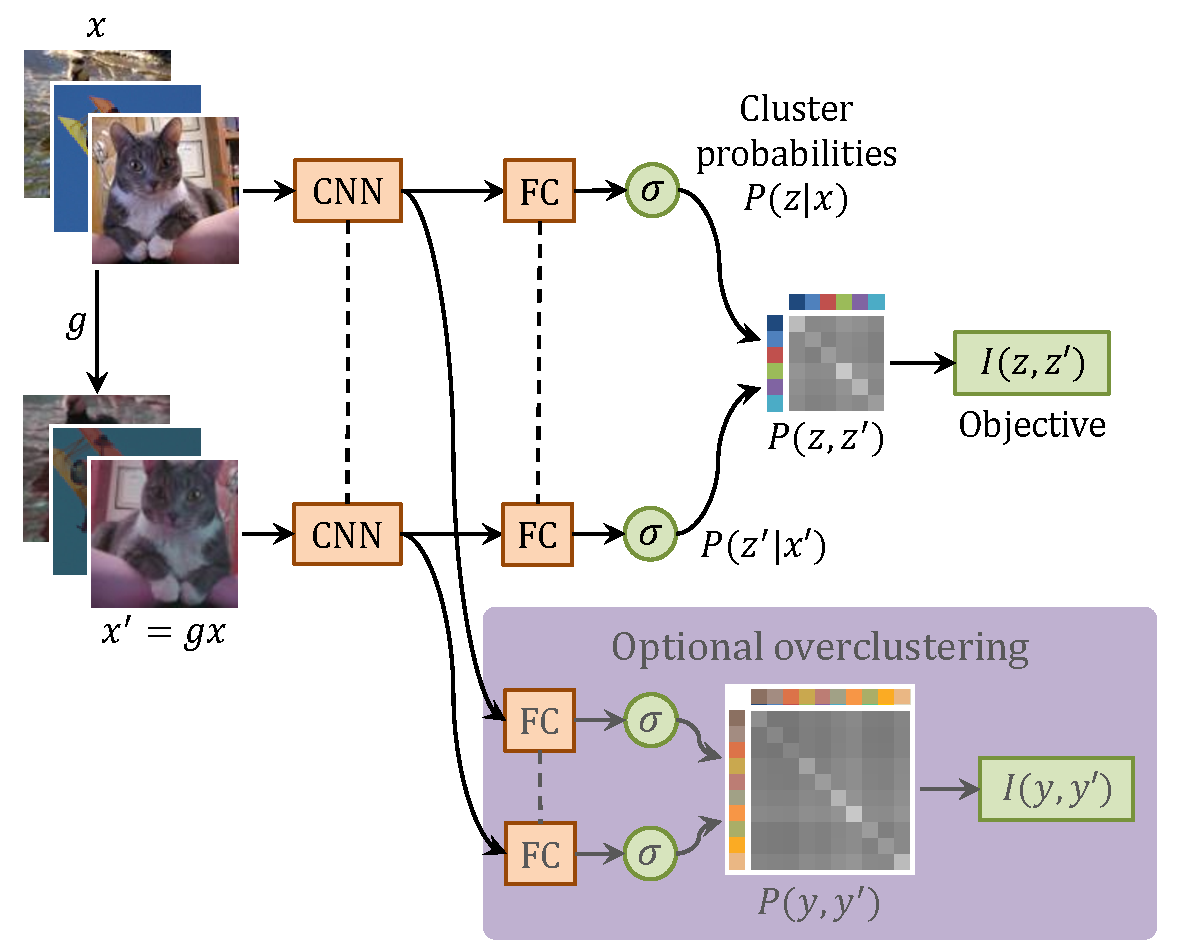
\includegraphics[width=0.95\columnwidth]{paper_imgs/overview1.pdf}
\caption{\label{f:overview}\methodnameshort for image clustering. Dashed line denotes shared parameters, $g$ is a random transformation, and $I$ denotes mutual information~(\cref{e:loss_expanded}).}
\end{figure}


\begin{figure*}
%\captionsetup{justification=centering}
\setlength\tabcolsep{2.2pt} % default value: 6pt

\begin{tabular}{c c c c c c}
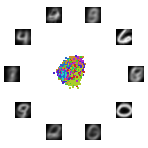
\includegraphics[height=0.16\textwidth]{experiments2_files/mnist_progression/726_run_1_colour_0_pointcloud_0.png} & 
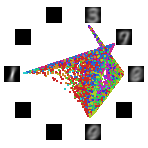
\includegraphics[height=0.16\textwidth]{experiments2_files/mnist_progression/726_run_1_colour_0_pointcloud_3.png} & 
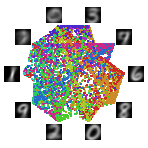
\includegraphics[height=0.16\textwidth]{experiments2_files/mnist_progression/726_run_1_colour_0_pointcloud_10.png} & 
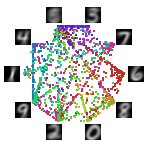
\includegraphics[height=0.16\textwidth]{experiments2_files/mnist_progression/726_run_1_colour_0_pointcloud_30.png} & 
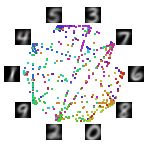
\includegraphics[height=0.16\textwidth]{experiments2_files/mnist_progression/726_run_1_colour_0_pointcloud_101.png} & 
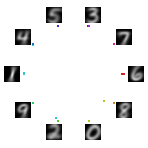
\includegraphics[height=0.16\textwidth]{experiments2_files/mnist_progression/726_run_1_colour_0_pointcloud_1000.png} 
\end{tabular}

\caption{\label{f:mnist_dots} Training with \methodnameshort on unlabelled MNIST in successive epochs from random initialisation (left). The network directly outputs cluster assignment probabilities for input images, and each is rendered as a coordinate by convex combination of 10 cluster vertices. There is no cherry-picking as the entire dataset is shown in every snapshot. Ground truth labelling (unseen by model) is given by colour. At each cluster the average image of its assignees is shown. With neither labels nor heuristics, the clusters discovered by \methodnameshort correspond perfectly to unique digits, with one-hot certain prediction (right).}
\end{figure*}


\paragraph{Co-clustering and mutual information.}

The use of information as a criterion to learn representations is not new. One of the earliest works to do so is by Becker and Hinton~\cite{becker1992self}.
More generally, learning from paired data has been explored in co-clustering~\cite{hartigan1972direct, dhillon2003information} and in other works~\cite{wang2010information} that build on the information bottleneck principle~\cite{friedman2001multivariate}.

Several recent papers have used information as a tool to train deep networks in particular.
IMSAT~\cite{hu2017learning} maximises mutual information between data and its representation and DeepINFOMAX~\cite{hjelm2018learning} maximizes information between spatially-preserved features and compact features.
However, IMSAT and DeepINFOMAX combine information with other criteria, whereas in our method information is the only criterion used.
Furthermore, both IMSAT and DeepINFOMAX compute mutual information over continuous random variables, which requires complex estimators~\cite{belghazi2018mine}, whereas \methodnameshort does so for discrete variables with simple and exact computations.
Finally, DeepINFOMAX considers the information $I(\bx, f(\bx))$ between the features $\bx$ and a deterministic function $f(\bx)$ of it, which is in principle the same as the entropy $H(\bx)$; in contrast, in \methodnameshort information does not trivially reduce to  entropy.

\paragraph{Semantic clustering versus intermediate representation learning.}
In semantic clustering, the learned function directly outputs discrete assignments for high level (i.e. semantic) clusters. Intermediate representation learners, on the other hand, produce continuous, distributed, high-dimensional representations that must be post-processed, for example by k-means, to obtain the discrete low-cardinality assignments required for unsupervised semantic clustering. The latter includes objectives such as generative autoencoder image reconstruction~\cite{vincent2010stacked},  triplets~\cite{schultz2004learning} and spatial-temporal order or context prediction~\cite{lee2017unsupervised,cruz2017deeppermnet,doersch2015unsupervised}, for example predicting patch proximity~\cite{isola2015learning}, solving jigsaw puzzles~\cite{noroozi2016unsupervised} and inpainting~\cite{pathak2016context}. Note it also includes a number of clustering methods (DeepCluster~\cite{caron2018deep}, exemplars~\cite{dosovitskiy2015discriminative}) where the clustering is only auxiliary; a clustering-style objective is used but does not produce groups with semantic correspondence. For example, DeepCluster~\cite{caron2018deep} is a state-of-the-art method for learning highly-transferable intermediate features using overclustering as a proxy task, but does not automatically find semantically meaningful clusters. As these methods use auxiliary objectives divorced from the semantic clustering objective, it is unsurprising that they perform worse than \methodnameshort~(\cref{s:experiments}), which directly optimises for it, training the network end-to-end with the final clusterer implicitly wrapped inside.




\paragraph{Optimising image-to-image distance.}

Many approaches to deep clustering, whether semantic or auxiliary, utilise a distance function between input images that approximates a given grouping criterion.
Agglomerative clustering~\cite{bautista2016cliquecnn} and partially ordered sets~\cite{bautista2017deep} of HOG features~\cite{dalal2005histograms} have been used to group images, and exemplars~\cite{dosovitskiy2015discriminative} define a group as a set of random transformations applied to a single image. Note the latter does not scale easily, in particular to image segmentation where a single $200\times 200$ image would call for 40k classes. DAC~\cite{chang2017deep}, JULE~\cite{yang2016joint}, DeepCluster~\cite{caron2018deep}, ADC~\cite{haeusser2018associative} and DEC~\cite{xie2016unsupervised} rely on the inherent visual consistency and disentangling properties~\cite{greff2015binding} of CNNs to produce cluster assignments, which are processed and reinforced in each iteration. 
The latter three are based on k-means style mechanisms to refine feature centroids, which is prone to degenerate solutions~\cite{caron2018deep} and thus needs explicit prevention mechanisms such as pre-training, cluster-reassignment or feature cleaning via PCA and whitening~\cite{xie2016unsupervised, caron2018deep}.

\begin{comment}
DAC is the only unsupervised clustering algorithm out of these that eschews k-means and agglomerative clustering for a different but similar clustering scheme, based on feature inner-products rather than distances.
DAC forms clusters gradually, in a self-paced manner, thus alleviating but not eliminating the risk of incurring degenerate solutions.
Furthermore, the nature of the optimisation, which reinforces bootstrapped class labels, creates a strong dependency on initialisation.

For unsupervised feature learning in general, i.e.\ where the training objective is not clustering, a large number of works explore using proxy learning tasks. 
There are two major directions:  generative tasks such as autoencoder image reconstruction~\cite{vincent2010stacked}, and spatial-temporal order or context prediction~\cite{lee2017unsupervised,cruz2017deeppermnet,doersch2015unsupervised}. The latter includes predicting patch proximity~\cite{isola2015learning}, solving jigsaw puzzles~\cite{noroozi2016unsupervised} and inpainting~\cite{pathak2016context}. 
In many cases they benefit from principled formulations that protect against degeneracy.
However, unlike the aforementioned clustering methods, the features learned by these methods need to be post-processed, for example using k-means, to cluster the data. 

\end{comment}

\paragraph{Invariance as a training objective.}

Optimising for function outputs to be persistent through spatio-temporal or non-material distortion is an idea shared by \methodnameshort with several works, including exemplars~\cite{dosovitskiy2015discriminative}, IMSAT~\cite{hu2017learning}, proximity prediction~\cite{isola2015learning}, the denoising objective of Tagger~\cite{greff2016tagger}, temporal slowness constraints~\cite{zou2012deep}, and optimising for features to be invariant to local image transformations~\cite{sohn2012learning,hui2013direct}.
More broadly, the problem of modelling data transformation has received significant attention in deep learning, one example being the transforming autoencoder~\cite{hinton2011transforming}.


% \section{Related work}\label{s:related}

% \paragraph{Co-clustering and mutual information.}

% The idea of learning a data representation by seeking the common parts of related observations is not new. 
% An early work is Becker and Hinton~\cite{becker1992self}, which maximises agreement between representations of 2D images to learn depth, using an objective corresponding to maximising mutual information between the input and the average of the data representations. 
% Co-learning has also been explored in the context of clustering by co-clustering methods, dating back to the pioneering work of Hartigan~\cite{hartigan72direct}. 
% Many information-theoretic variant of such approaches have been proposed, as discussed by~\cite{wang10information}, which are generally related to the information bottleneck principle~(\cite{friedman2001multivariate}). 

% A few works have employed mutual information in the context of unsupervised deep learning. IMSAT~\cite{hu2017learning} maximises mutual information between input data and their predicted discrete representations whilst encouraging the representations of augmented data points to be close to those of the original data points. 
% DeepINFOMAX~\cite{hjelm2018learning} maximises mutual information between spatially preserved features and compact features. There are some major differences with \methodnameshort. 
% Firstly, mutual information is used as an aid in these methods, as it increases the statistical predictivity between two random variables. 
% This contrasts with our method, where mutual information constitutes the loss applied directly to cluster assignments, meaning it is used as a clustering objective. 
% Secondly, both IMSAT and DeepINFOMAX compute mutual information over continuous random variables, which calls for an integral and is not computationally tractable, so estimators~\cite{belghazi2018mine} are used. 
% Since \methodnameshort maximises mutual information between cluster assignments and the number of clusters is discrete, computation is exact and straightforward. 
% Finally, DeepINFOMAX employs mutual information between function inputs and outputs, i.e. $I(x, f(x))$, but the conditional entropy component of mutual information $H(f(x) | x)$ is 0 when $f$ is deterministic, making the maximisation less meaningful. 
% In contrast \methodnameshort maximises mutual information between cluster assignments of separate images, i.e. $I(z, z')$ where $z$ and $z'$ are not functions of one other, making $H(z | z')$ a non-zero quantity that contributes to the optimisation as it can be minimised.

% \paragraph{Optimising image-to-image distance for clustering.}
% Many works for on unsupervised deep clustering involve establishing a scheme for estimating the semantic distance between input images, before training a function to learn this scheme. 
% CliqueCNN~\cite{bautista2016cliquecnn} trains a network to discriminate between cliques that are determined by applying agglomerative clustering on image features such as HOG~\cite{dalal2005histograms}. 
% In Exemplar CNNs~\cite{dosovitskiy2016discriminative}, each image and a its set of random transformations is considered a class, and a function is trained to discriminate between these surrogate classes. Like \methodnameshort, this method uses random transformations as a proxy for obtaining images with low semantic distance in the absence of label information. 
% Requiring one class per input image has a large memory footprint which makes Exemplar CNNs infeasible for segmentation (where patches are clustered instead of images, so a single 200x200 image would call for 40k classes). 

% \begin{figure}[t]
\centering
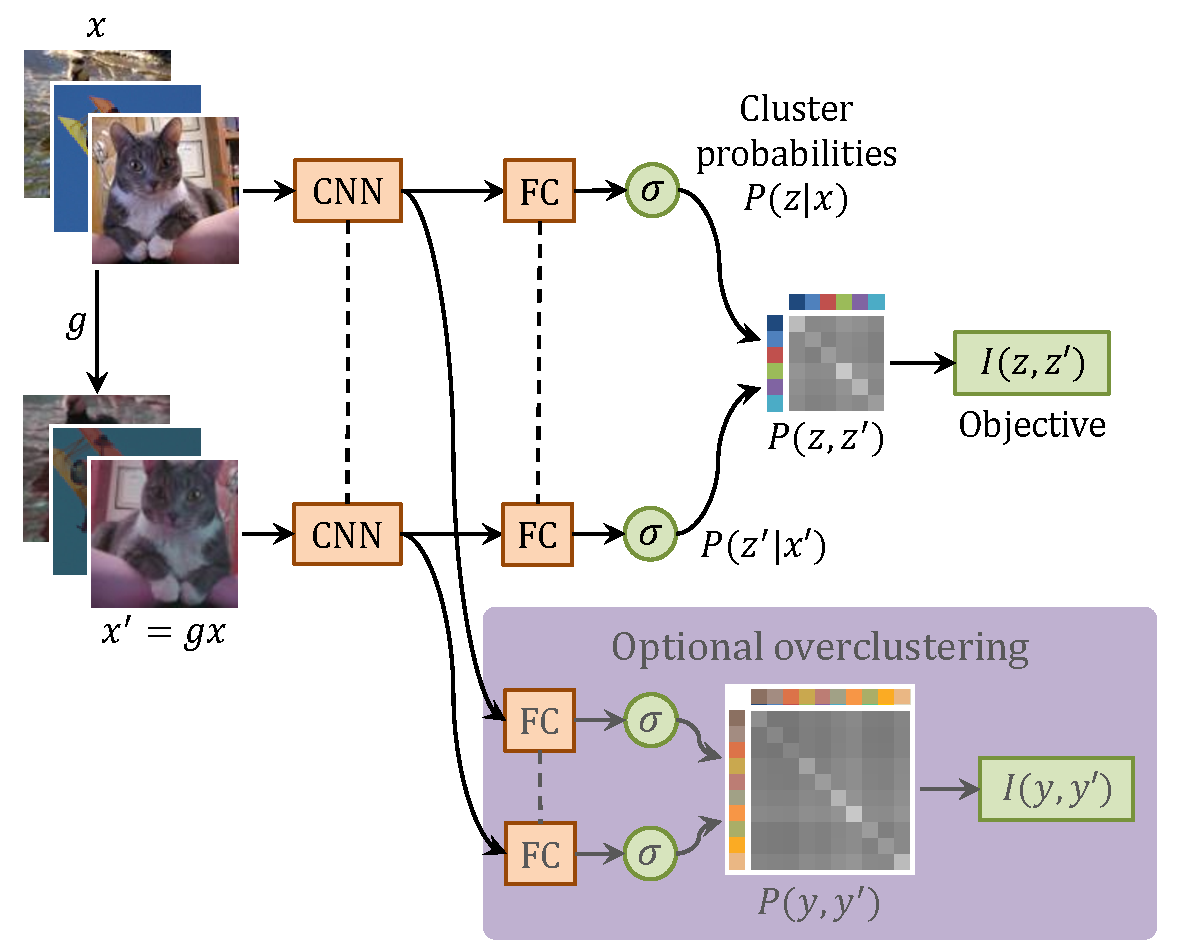
\includegraphics[width=0.95\columnwidth]{paper_imgs/overview1.pdf}
\caption{\label{f:overview}\methodnameshort for image clustering. Dashed line denotes shared parameters, $g$ is a random transformation, and $I$ denotes mutual information~(\cref{e:loss_expanded}).}
\end{figure}


% DAC~\cite{chang2017deep}, JULE~\cite{yang2016joint}, DeepCluster~\cite{caron2018deep}, Associative Deep Clustering~\cite{haeusser18associative} and DEC~\cite{xie2016unsupervised} all rely on the inherent visual consistency and disentangling properties~\cite{greff2015binding} of CNNs to produce meaningful cluster assignments, which are processed and reinforced in each iteration. 
% The latter three are based on using k-means to refine deep feature vectors, a mechanism which is prone to degenerate solutions~\cite{caron2018deep} and thus needs explicit prevention mechanisms such as pre-training, cluster-reassignment or feature cleaning via PCA and whitening ~\cite{xie2016unsupervised, caron2018deep}. 

% DAC is the only unsupervised clustering algorithm out of these that eschews k-means whilst training a network to directly produce cluster assignments, as \methodnameshort does. 
% A network is trained to produce cluster assignment probability distributions for each sample that are used as high level feature descriptors, and the dot product of different descriptors is treated as a proxy for inter-sample semantic distance (instead of Euclidian distance, which is used in the k-means based clusterers). 
% Training proceeds by maximising the dot product of close sample pairs, thus encouraging them to be assigned to the same cluster, whilst minimising the dot product for far pairs. 
% The nature of the optimisation means there is a strong dependency on initialisation and lack of protection against degenerate solutions such as clusters disappearing. 

% \paragraph{Proxy tasks for unsupervised feature learning.}
% For unsupervised feature learning in general, i.e. where the training objective is not clustering, a large number of works explore using proxy learning tasks. 
% There are two major camps:  generative tasks such as autoencoder image reconstruction~\cite{vincent2010stacked}, and spatial-temporal order or context prediction~\cite{lee2017unsupervised,cruz2017deeppermnet,doersch2015unsupervised}. The latter includes predicting patch proximity~\cite{isola2015learning}, solving jigsaw puzzles~(\cite{noroozi2016unsupervised}) and inpainting~(\cite{pathak2016context}). 
% In many cases they benefit from principled formulations that protect against degeneracy.
% However, unlike the aforementioned clustering methods, learned representations from these tasks constitute fine-grained continuous features rather than coarse cluster assignments, and thus must be post-processed, either by unsupervised clustering such as k-means or with label information via SVMs or fine-tuning, in order to produce semantic clusters.

% \paragraph{Invariance as a training objective.}
% Training for function outputs to be persistent through spatio-temporal distortion, noise distortion, or random transforms is an idea shared by \methodnameshort and several mentioned works, including Exemplar CNNs~\cite{dosovitskiy2016discriminative}, IMSAT~\cite{hu2017learning} and proximity prediction~\cite{isola2015learning}.
% It is also seen in Tagger~\cite{greff2016tagger}, which trains a function to denoise its input using several clusters to distribute the representation,~\cite{zou2012deep} which enforces a temporal slowness constraint on learned features, and~\cite{sohn2012learning,hui2013direct} which train for features invariant to local image transformations.




\section{Problem and Notations}
\label{sec:problem_definition}
Given RGB-D data as input, our goal is to classify and localize objects in 3D space. The depth data, obtained from LiDAR or indoor depth sensors, is represented as a point cloud in RGB camera coordinates. The projection matrix is also known so that we can get a 3D frustum from a 2D image region. Each object is represented by a class (one among $k$ predefined classes) and an \emph{amodal} 3D bounding box. The \emph{amodal} box bounds the complete object even if part of the object is occluded or truncated. The 3D box is parameterized by its size $h,w,l$, center $c_x, c_y, c_z$, and orientation $\theta, \phi, \psi$ relative to a predefined canonical pose for each category. In our implementation, we only consider the heading angle $\theta$ around the up-axis for orientation.

\section{Approach}
\subsection{Overview}

% \todo{
% the challenge of point cloud representation; from a high-level, how we are able to overcome the challenge
% 
% aside, the ambiguity of groundtruth is an inherent property of this problem; how do we resolve this problem.
% 
% describe the overall network architecture; give the road map for the rest of the section.
% }

Our task of building a conditional generative network for point sets is challenging, due to the unordered form of representation and the inherent ambiguity of groundtruth. These challenges has pushed us to invent new architecture, loss function, and learning paradigm. Specifically, we have to address three subproblems: 

\para{Point set generator architecture}: Network to predict point set is barely studied in literature, leaving a huge open space for us to explore the design choices. Ideally, a network should make the best use of its data statistics and possess enough representation power. We propose a network with two prediction branches, one enjoys high flexibility in capturing complicated structures and the other exploits geometric continuity. Its representation power is further boosted by an hourglass structure. See Sec~\ref{sec:method:network}. 

\para{Loss function for point set comparison}: For our novel type of prediction, point set, it is unclear how to measure the distance between the prediction and groundtruth. We introduce two distance metrics for point sets -- the Chamfer distance and the Earth Mover's distance. We show that both metrics are differentiable almost everywhere and can be used as the loss function, but has different properties in capturing shape space. See Sec~\ref{sec:method:loss}.

\para{Modeling the uncertainty of groundtruth}: Our problem of 3D structural recovery from a single image is ill-posed, thus the ambiguity of groundtruth arises during the train and test time. It is fundamentally important to characterize the ambiguity of groundtruth for a given input, and practically desirable to be able to generate multiple predictions. Surprisingly, this goal can be achieved tactfully by simply using the $\min$ function as a wrapper to the above proposed loss, or by a conditional variational autoencoder.  See Sec~\ref{sec:method:gan}.
% The form of the wrapper function is a $\min$ function of $n$ numbers. 
% The learning of this wrapped loss function (named {\bf MoN} loss) is almost as efficient and easy as the original one. 

% Here we choose the point cloud representation for 3D shapes --  a shape is a set of 3D coordinates $\mathcal{S}=\{(x_1, y_1, z_1),\dots, (x_n, y_n, z_n)\}$. By set, we mean a collection of \emph{orderless} entities.

% Most deep learning work predict either sequential data or 2D/3D arrays, thus there lacks literature on how point set should be represented and predicted. 

% Different from previous 3D deep learning work such as  that represent shapes by volume,
% Our system takes a single RGB or depth image as input, and is able to predict a list of a complete 3D point set as the candidate underlying 3D shape.

\subsection{Point Set Prediction Network}
\label{sec:method:network}
% \todo{
% describe the basic architecture of the point set predictor network;
% 
% describe the hour-glass network structure
% 
% describe the use of deconv branch and fc branch;
% }
The task of building a network for point set prediction is new. We design a network with the goal of possessing strong representation power for complicated structures, and make the best use of the statistics of geometric data. 
 % Next we introduce the basic ideas behind of our proposed network architecture. 
To introduce our network progressively, we start from a simple version and gradually add components.

% Given an image and a random vector as input, our point set prediction network ({\bf PointOutNet}) outputs a set of $N$ points in $\R^3$. This set is represented as an $N\times 3$ matrix, whose each row corresponds to a point.

As in Fig~\ref{fig:pointnet} (top), our network has an encoder stage and a predictor stage. The encoder maps the input pair of an image $\image$ and a random vector $r$ into an embedding space. The predictor outputs a shape as an $N\times 3$ matrix ${\bf M}$, each row containing the coordinates of one point.

The encoder is a composition of convolution and ReLU layers; in addition, a random vector $r$ is subsumed so that it perturbs the prediction from the image $I$. We postpone the explanation of how $r$ is used to Sec~\ref{sec:method:gan}. %This is done by first converting $r$ into a 3-dimensional tensor through fully-connected layers and a reshape layer, and then concatenating this tensor with the feature map of $I$, as in our supplementary. 
The predictor generates the coordinates of $N$ points through a fully connected network. Though simple, this version works reasonably well in practice. 

We further improve the design of the predictor branch to better accommodate large and smooth surfaces which are common in natural objects. The fully connected predictor as above cannot make full use of such natural geometric statistics, since each point is predicted independently. The improved predictor in Fig~\ref{fig:pointnet} (middle) exploits this geometric smoothness property. 

This version has two parallel predictor branches -- a fully-connected (fc) branch and a deconvolution (deconv) branch. The fc branch predicts $N_1$ points as before. The deconv branch predicts a 3 channel image of size $H\times W$, of which the three values at each pixel are the coordinates of a point, giving another $H\times W$ points. Their predictions are later merged together to form the whole set of points in ${\bf M}$. Multiple skip links are added to boost information flow across encoder and predictor. 

With the fc branch, our model enjoys high flexibility, showing good performance at describing intricate structures. With the deconvolution branch, our model becomes not only more parameter parsimonious by weight sharing; but also more friendly to large smooth surfaces, due to the spatial continuity induced by deconv and conv. Refer to Sec~\ref{sec:exp:analysis} for experimental evidences. 

To pursue even better performance, we introduce the hourglass version in Fig~\ref{fig:pointnet} (bottom), inspired by \cite{newell2016stacked}. This deep network conducts the encoding-decoding operations recurrently, thus has stronger representation power and can mix global and local information better. 

Above introduces the design of our network $\mathbb{G}$ in Eq~\ref{eqn:main}. To train this network, however, we still need to design a proper loss function for point set prediction, and enable the role $r$ for multiple candidates prediction. We explain in the next two sections.
\subsection{Distance Metric between Point Sets}
\label{sec:method:loss}



A critical challenge is to design a good loss function for comparing the predicted point cloud and the groundtruth. To plug in a neural network, a suitable distance must satisfy at least three conditions: 1) differentiable with respect to point locations; 2) efficient to compute, as data will be forwarded and back-propagated for many times; 3) robust against small number of outlier points in the sets (e.g. Hausdorff distance would fail).

We seek for a distance $d$ between subsets in $\R^3$, so that the loss function $L(\{S^{pred}_i\}, \{S^{gt}_i\})$ takes the form
\begin{align}
    L(\{S^{pred}_i\}, \{S^{gt}_i\}) = \sum d(S^{pred}_i, S^{gt}_i),
    \label{eqn:loss}
\end{align}
where $i$ indexes training samples, $S_i^{pred}$ and $S_i^{gt}$ are the prediction and groundtruth of each sample, respectively.

We propose two candidates: Chamfer distance (CD) and Earth Mover's distance (EMD)~\cite{rubner2000earth}.

\paragraph{Chamfer distance} We define the Chamfer distance between $S_1, S_2\subseteq \R^3$ as:
\begin{align*}
%\mathbb{D}_{\mbox{CD}}(S_1, S_2)=\frac{1}{|S_1|}\sum_{x\in S_1} \min_{y\in S_2} \|x-y\|_2+\frac{1}{|S_2|}\sum_{y\in S_2} \min_{x\in S_1} \|x-y\|_2
d_{CD}(S_1, S_2)=\sum_{x\in S_1}\min_{y\in S_2} \|x-y\|^2_2+\sum_{y\in S_2}\min_{x\in S_1} \|x-y\|^2_2
\end{align*}
In the strict sense, $d_{CD}$ is not a distance function because triangle inequality does not hold. We nevertheless use the term ``distance'' to refer to any non-negative function defined on point set pairs. For each point, the algorithm of CD finds the nearest neighbor in the other set and sums the squared distances up.   Viewed as a function of point locations in $S_1$ and $S_2$, $\mbox{CD}$ is continuous and piecewise smooth. The range search for each point is independent, thus trivially parallelizable. Also, spatial data structures like KD-tree can be used to accelerate nearest neighbor search. Though simple, CD produces reasonable high quality results in practice.

\paragraph{Earth Mover's distance} 

Consider $S_1, S_2\subseteq \R^3$ of equal size $s=|S_1|=|S_2|$. The EMD between $A$ and $B$ is defined as:
\begin{align*}
d_{EMD}(S_1, S_2)=\min_{\phi:S_1\rightarrow S_2} \sum_{x\in S_1} \|x-\phi(x)\|_2
\end{align*}
where $\phi:S_1\rightarrow S_2$ is a bijection.

The EMD distance solves an optimization problem, namely, the assignment problem. For all but a zero-measure subset of point set pairs, the optimal bijection $\phi$ is unique and invariant under infinitesimal movement of the points. Thus EMD is differentiable almost everywhere. In practice, exact computation of EMD is too expensive for deep learning, even on graphics hardware. We therefore implement a $(1+\epsilon)$ approximation scheme given by \cite{bertsekas1985distributed}. We allocate fix amount of time for each instance and incrementally adjust allowable error ratio to ensure termination. For typical inputs, the algorithm gives highly accurate results (approximation error on the magnitude of $1\%$). The algorithm is easily parallelizable on GPU.

%\paragraph{Shape space} Though more expensive to compute, the shape space induced by EMD is nicer than by CD. Fig~\ref{fig:interoplation} illustrates their differences in a shape interpolation simulation. Evidently, the mean shape by EMD is cleaner and clearer in structure. Intuitively, this is because the EMD is obtained through solving a point-wise correspondence problem, and the correspondence implicitly suggests the proper movement of each point for interpolation. In contrast, the mean shape from CD is more splashy, as CD takes a greedy algorithm (nearest neighbor) to match points, resulting in a strategy that tends to hedge the uncertainty in groundtruth by a few isolated points. 

%We are particularly interested in how point clouds will be averaged, because this precursors what our complicated network may learn. As will be discussed in more detail in the next section, 3D reconstruction from a single 2D image is inherently ambiguous. Such ambiguity affects the optimization of loss function (Eq~\ref{eqn:loss}), an objective that drives to average possible groundtruth shapes for each input. 

%In 3D reconstruction experiments, we do observe similar trends: Chamfer distance tends to induce a more ``aggressive'' reconstruction by placing a few points at uncertain space; in contrast, EMD tends to be more conservative and produce less spurious points.

%\begin{figure}[t!]
  %\centering
  %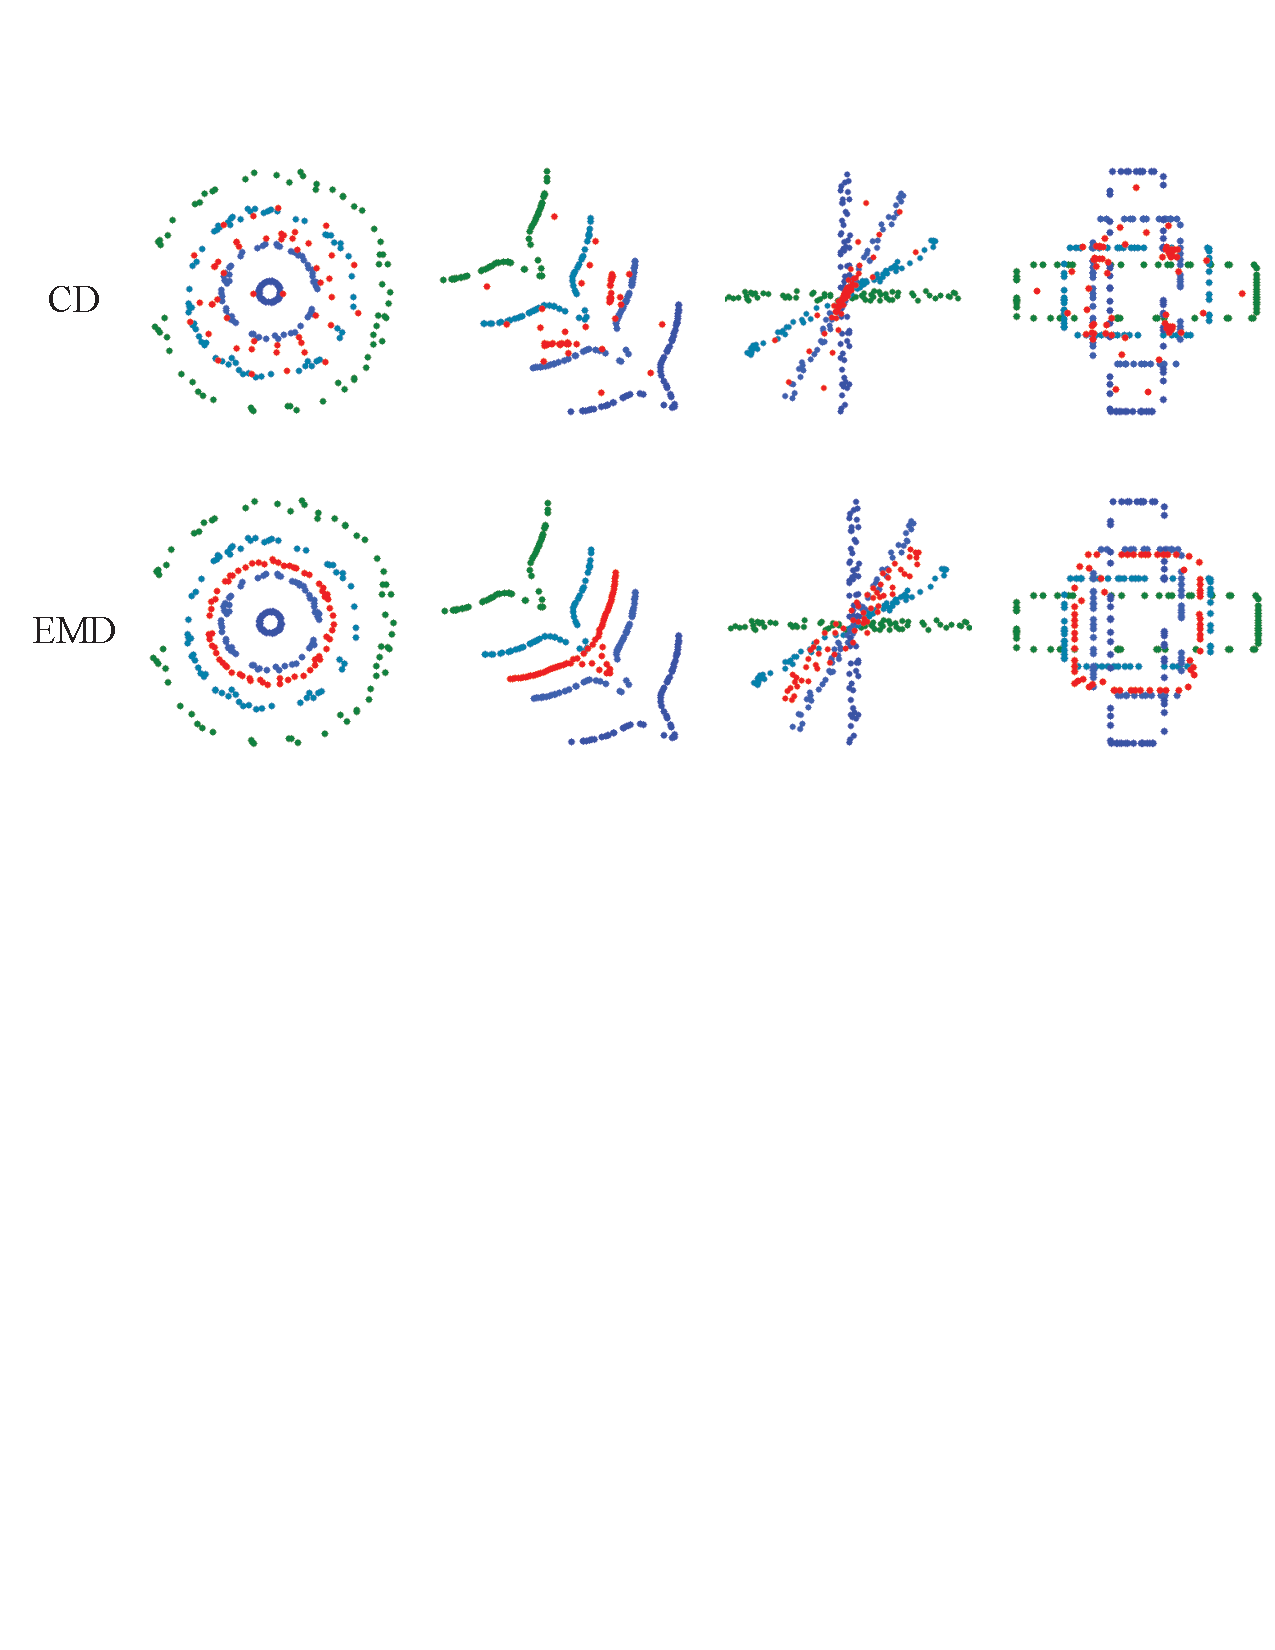
\includegraphics[width=\linewidth]{./fig/interpolation}
  %\caption{The interpolation of point sets by Chamfer distance (CD) versus Earth %Mover's distance (EMD). Each column corresponds to one type of shape. For each %type, we compute the mean shape $E$ (red) from four samples $S_i$ with different %parameters (from green to blue), e.g., radius of a circle. The mean shape is %computed by solving the optimization problem $\min_E \sum_{i=1}^4 d^2(E, S_i)$, %where $d$ can be CD or EMD. We observe that the mean shape from EMD looks more %natural.}
  %\label{fig:interoplation}
%\end{figure}

\paragraph{Shape space}
Despite remarkable expressive power embedded in the deep layers, neural networks inevitably encounter uncertainty in predicting the precise geometry of an object. Such uncertainty could arise from limited network capacity, insufficient use of input resolution, or the ambiguity of groundtruth due to information loss in 3D-2D projection. Facing the inherent inability to resolve the shape precisely, neural networks tend to predict a ``mean'' shape averaging out the space of uncertainty. The mean shape carries the characteristics of the distance itself.

In Figure~\ref{fig:mean}, we illustrate the distinct mean-shape behavior of EMD and CD on synthetic shape distributions, by minimizing
% \begin{equation*}
% \begin{aligned}
% \underset{x}{\mbox{minimize}}&&\mathrm{E}_{s\sim S}[L(x,s)]
% \end{aligned}
% \end{equation*}
$\mathrm{E}_{s\sim \mathbb{S}}[L(x,s)]$
through stochastic gradient descent, where $\mathbb{S}$ is a given shape distribution, $L$ is one of the distance functions. 

In the first and the second case, there is a single continuously changing hidden variable, namely the radius of the circle in (a) and the location of the arc in (b). EMD roughly captures the shape corresponding to the mean value of the hidden variable. In contrast CD induces a splashy shape that blurs the shape's geometric structure. In the latter two cases, there are categorical hidden variables: which corner the square is located at (c) and whether there is a circle besides the bar (d). To address the uncertain presence of the varying part, the minimizer of CD distributes some points outside the main body at the correct locations; while the minimizer of EMD is considerably distorted.

\begin{figure}[t!]
\centering
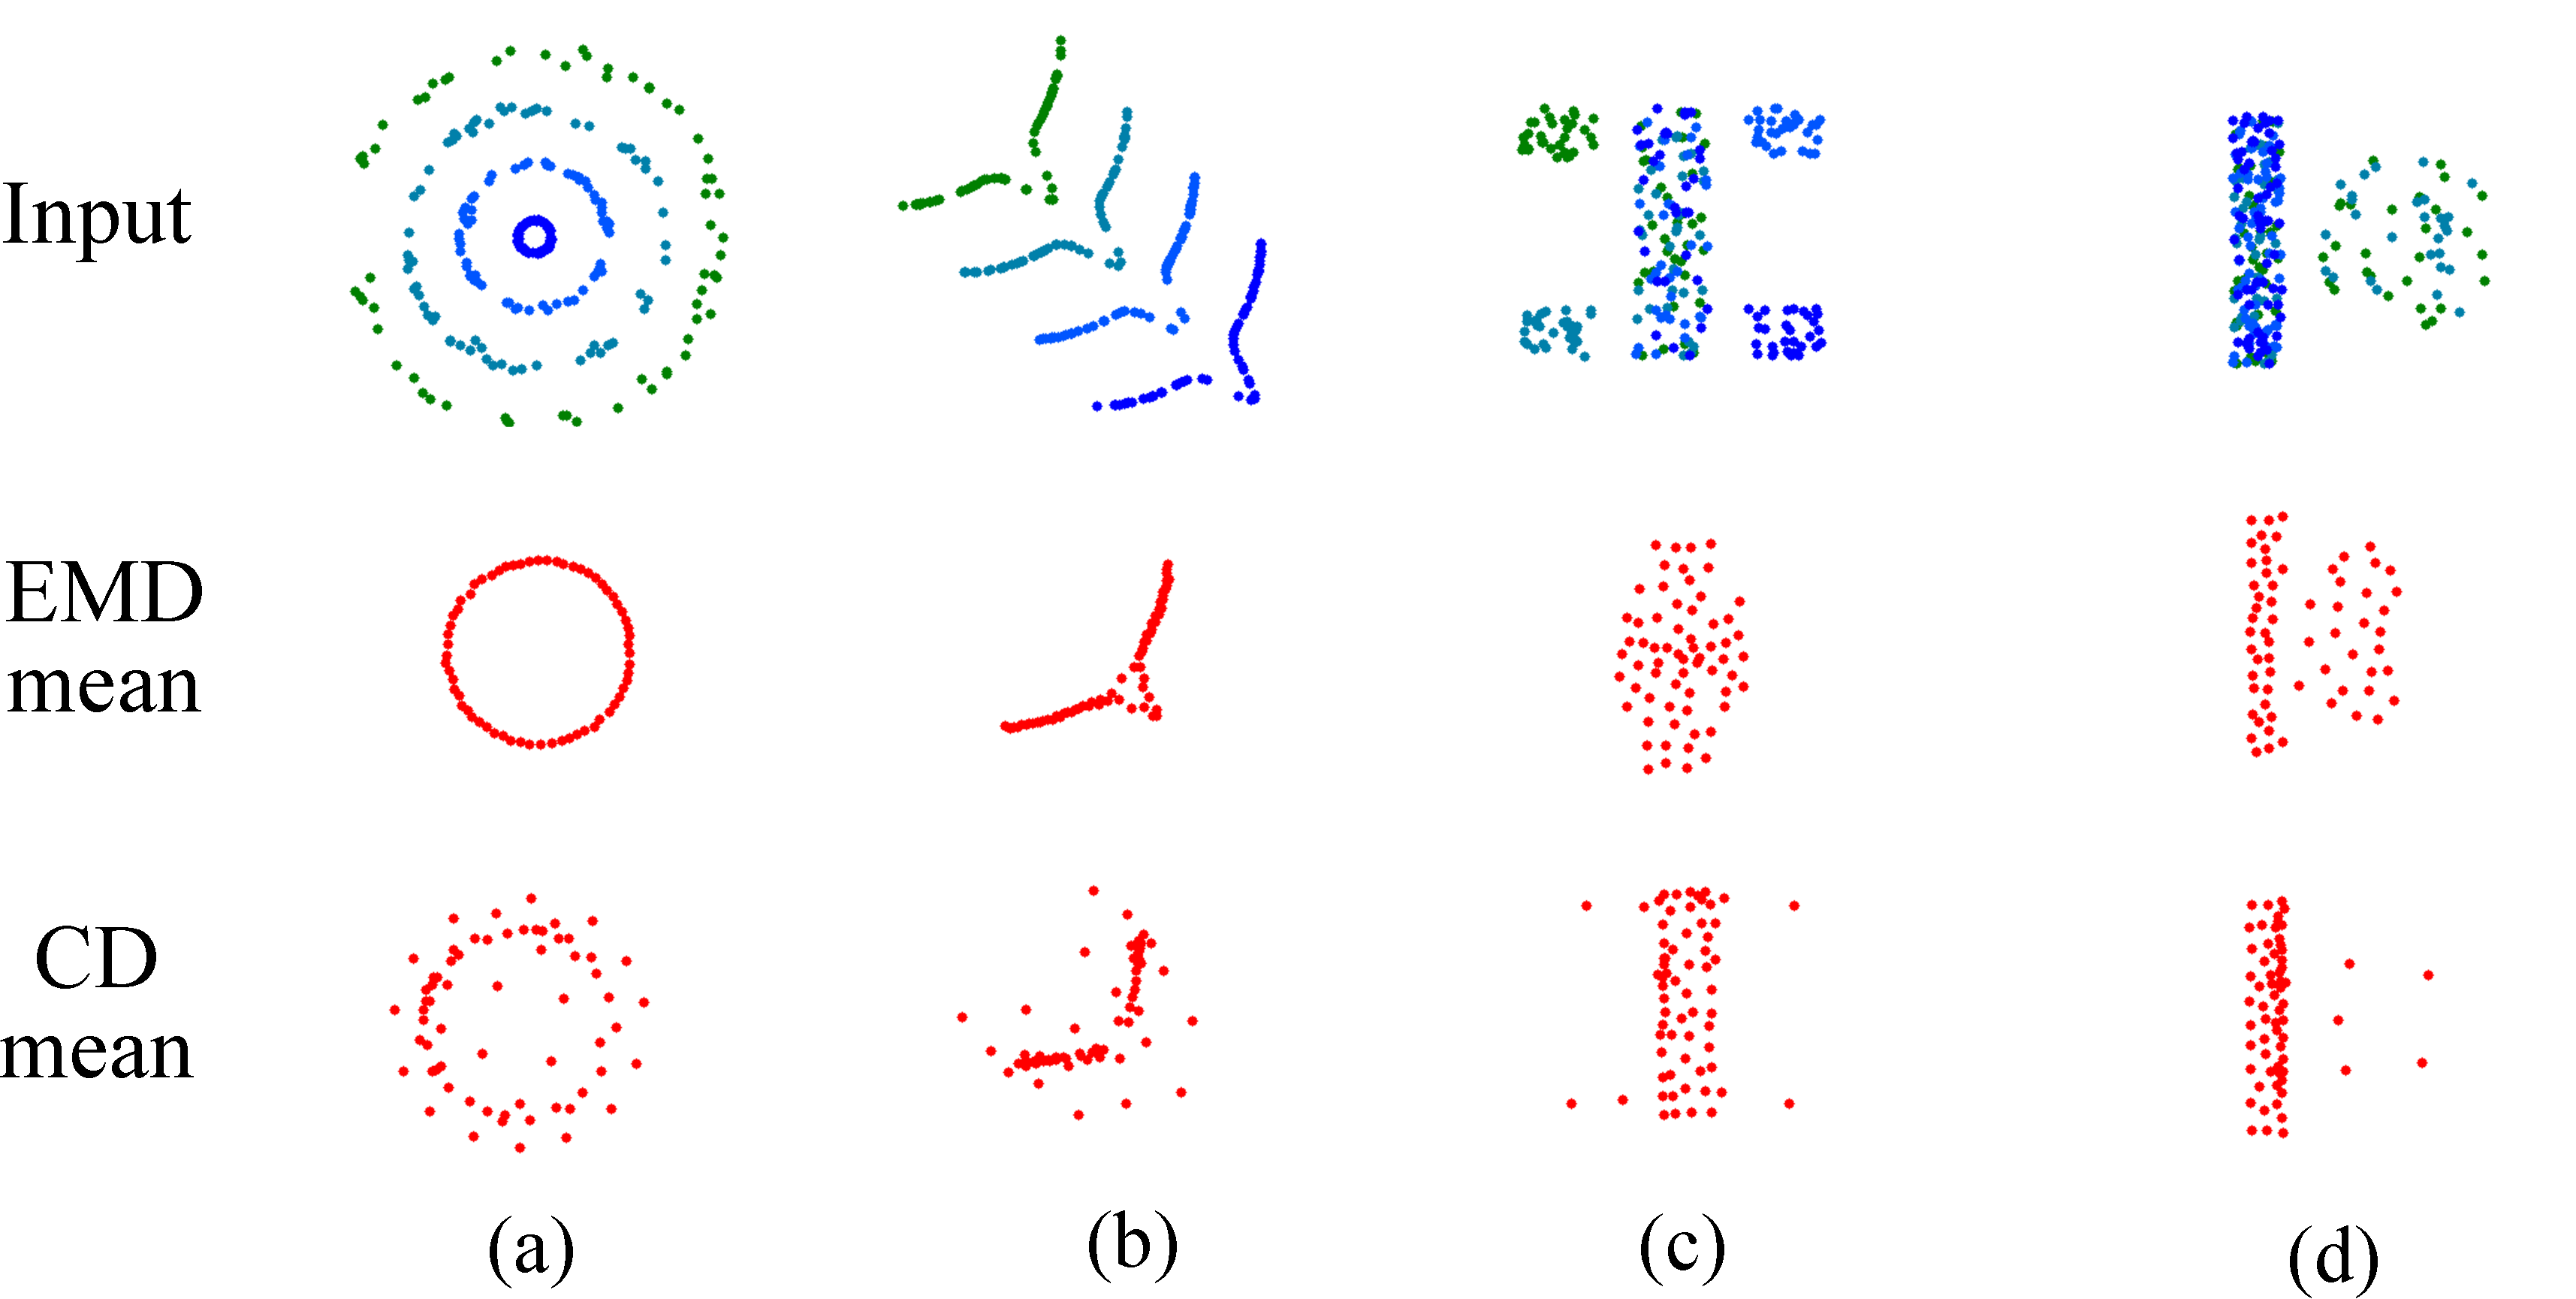
\includegraphics[width=0.9\linewidth]{./fig/show_mean.pdf}
\caption{Mean-shape behavior of EMD and CD. The shape distributions are (a) a circle with varying radius; (b) a spiky arc moving along the diagonal; (c) a rectangle bar, with a square-shaped attachment allocated randomly on one of the four corners; (d) a bar, with a circular disk appearing next to it with probability 0.5. The red dots plot the mean shape calculated according to EMD and CD accordingly.}
\label{fig:mean}
\end{figure}

\subsection{Generation of Multiple Plausible Shapes}
\label{sec:method:gan}
% \todo{
% this is an inherent property of our problem. give an illustrative example to convince the reader.
% 
% therefore, ideally, we should be able to generate the space of plausible shapes. we can think that the gt for each training data is just a sample from the groundtruth space. 
% 
% so we come up with the idea -- make multiple predictions, and at least one of the prediction should match the groundtruth.
% }

Our problem solves an ill-posed problem of 3D structural recovery from a single projection. Posed as a regression problem, ambiguity of the prediction arises at test time -- the depth for visible parts is under-determined, and the geometry for invisible parts has to be hallucinated by guessing. In a statistical view, reasonable predictions from the input image form a distribution.  Reflected in the training set, two images that look alike may have rather different groundtruth shapes. Recall the discussion in the previous section -- the ambiguity of groundtruth shape may significantly affect the trained predictor, as the loss function \eqref{eqn:loss} induces our model to predict the mean of possible shapes.  

\begin{figure}[t!]
  \centering
  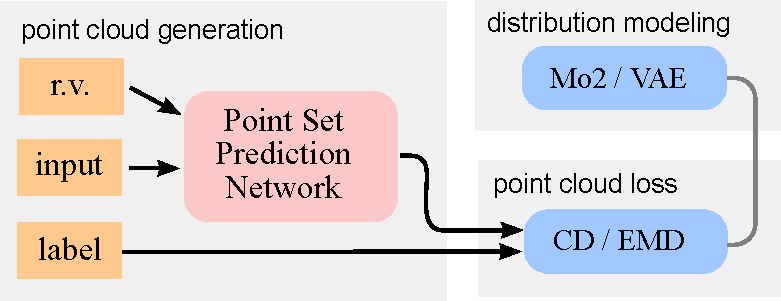
\includegraphics[width=0.8\linewidth]{./fig/system.pdf}
  \caption{System structure. By plugging in distributional modeling module, our system is capable of generating multiple predictions. }
  \label{fig:network}%xiao qiang zhen bang
\end{figure}
%ndeed, the nice interpolation ability of EMD helps us to generate a reasonable mean shape; however, ideally we should fully characterize the landscape of the groundtruth distribution, or be able to sample plausible candidates accordingly. Statistically, we are looking for a conditional sampler dependent on the input image. In this view, the groundtruth shape of each image provided by the training data is in fact a sample from the groundtruth distribution.

To better model the uncertainty or inherent ambiguity (e.g. unseen parts in the single view), we enable the system to generate distributional output. We expect that the random variable $r$ passed to $\mathbb{G}$ (see Eq~\eqref{eqn:main}) would help it explore the groundtruth distribution, in analogy to conditional GAN (CGAN)~\cite{mirza2014conditional}. However, naively plugging $\mathbb{G}$ from Eq~\eqref{eqn:main} into Loss~\eqref{eqn:loss} to predict $S_i^{pred}$ won't work, as the loss minimization will nullify the randomness. It is also unclear how to make CGAN work in our scenario, as building a discriminator that directly consumes a point set is itself an open problem. 

The problem can be solved by more complex frameworks like VAE, where we can incorporate secondary input channels (e.g. another view). However, we find practically a simple and effective method for uncertainty modeling: the MoN loss. We train our network by minimizing a loss function as below:
\begin{equation}
    \begin{aligned}
    \underset{\Theta}{\mbox{minimize}} 
    && 
    \sum_k 
        \min_{
            \substack{r_j\sim \mathbb{N}(\mathbf{0}, \mathbf{I})\\1\le j\le n}
        }
        \{
            d(\mathbb{G}(I_k, r_j;\Theta), S_k^{gt})
        \}
    \end{aligned} 
    \label{eqn:gan}
\end{equation}    

We explain the rationale behind Problem~\eqref{eqn:gan} here. Given an image $I_k$, $\mathbb{G}$ makes $n$ predictions by perturbing the input with $n$ random vectors $r_j$. Intuitively, we expect that one of the predictions will be close to the groundtruth $S_k^{gt}$ given by the training data, meaning that the minimum of the $n$ distances between each prediction and the groundtruth must be small. 

We name this loss as Min-of-N loss (MoN), since it comes from the minimum of $n$ distances. Any of the point set regression networks in Fig~\ref{fig:pointnet} can be plugged into the meta network in Fig~\ref{fig:network} incorporating the MoN loss. In practice, we find that setting $n=2$ already enables our method to well explore the groundtruth space.  Please refer to Sec~\ref{sec:exp:gan} for experiment results.

An alternative way to achieve the conditional shape sampler is by a conditional variational autoencoder. For more details about variational autoencoders, please refer to \cite{doersch2016tutorial}.  Fig~\ref{fig:VAE} shows the system architecture for training and testing a conditional variational autoencoder $P(S|X)$ in our case. Here, $X$ is the input image and $S$ is the \emph{point cloud} representation of the groundtruth 3D shape. At training time, each input image $X$ will be augmented by a random variable that is conditioned on $Y$, which takes the \emph{volumetric} representation of the groundtruth shape $S$. A 3D convolutional network is used as the encoder $Q$ (see \cite{maturana2015voxnet} for a good reference of 3D conv networks). Therefore, a local proximity in the embedding space contains the variations of possible groundtruth 3D shapes.

\begin{figure}
\centering
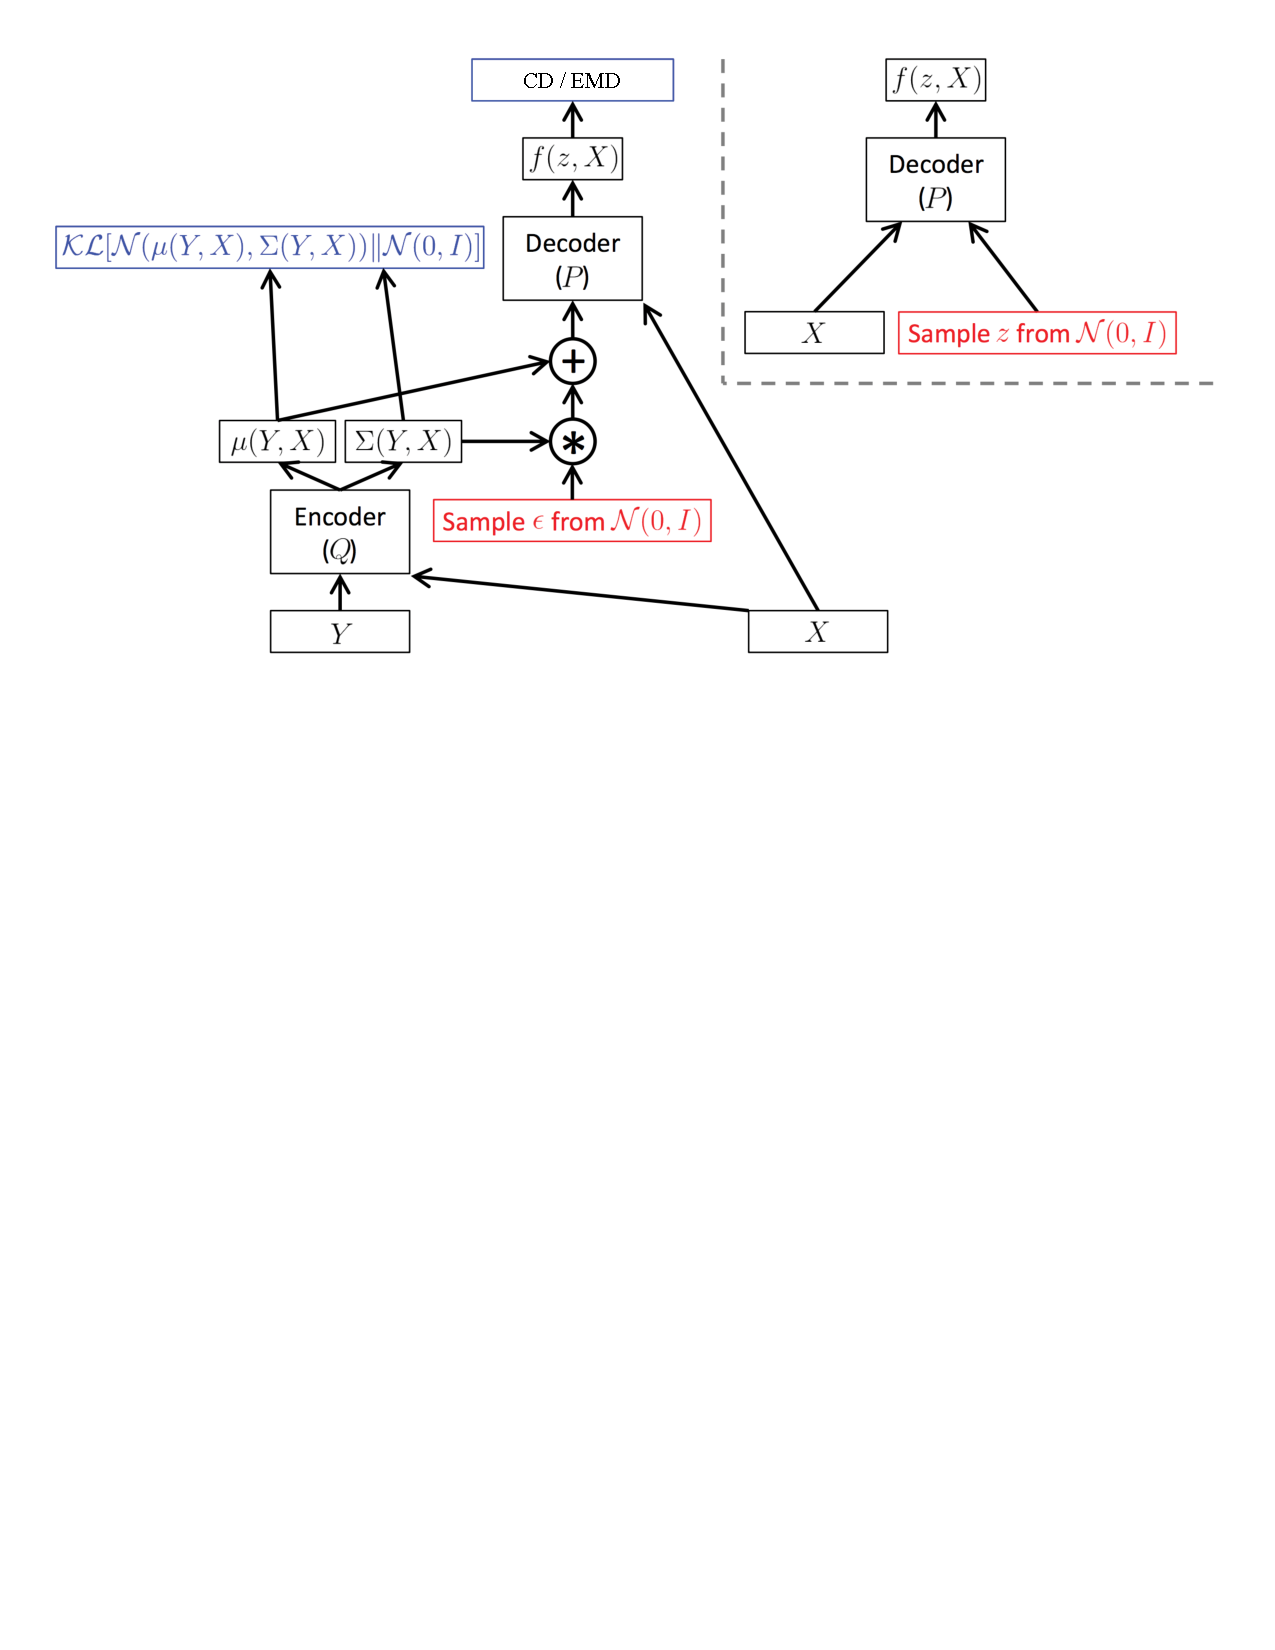
\includegraphics[width=\linewidth]{./fig/vae.pdf}
\caption{Network for conditional variational autoencoder shape sampler $P(S|X)$. Left: a training-time conditional variational autoencoder implemented as a feedforward neural network. Here, $Y$ is the volumetric form of the groundtruth shape $S$, whereas $f(z, X)$ is the point cloud form of the predicted shape for $S$. Right: the same model at test time. (Modified from Doersch et al.~\cite{doersch2016tutorial})}
\label{fig:VAE}
\end{figure}

% An alternative way to build the conditional sampler is through conditional variational autoencoder (VAE) technique, which requires a few additional modules. We explain the VAE version in the supplementary. 





\section{Experiment}
\section{Evaluation}
In this section, we present a comparative performance evaluation of our proposed method.
Specifically, we conduct experiments on the widely-used fine-grained benchmark Caltech-UCSD birds dataset \cite{DatasetCUB200} (CUB200-2011).
The classification task is to discriminate among 200 species of birds, and is challenging for computer vision systems due to the high degree of similarity between categories.
It contains 11,788 images of 200 bird species. Each image is annotated with its bounding box and the image coordinates of fifteen keypoints: the beak, back, breast, belly, forehead, crown, left eye, left leg, left wing, right eye, right leg, right wing, tail, nape and throat. We train and test on the splits included with the dataset, which contain around 30 training samples for each species.
Following the protocol of \cite{dpd}, we use two semantic parts for the bird dataset: head and body.
%Figure~\ref{fig:ningfig} (left) illustrates the set of keypoints which comprise the head part, and Figure~\ref{fig:ningfig} (right) illustrates the body part.

We use the open-source package Caffe~\cite{Jia13caffe} to extract deep features and fine-tune our CNNs. For object and part detections, we use the Caffe reference model, which is almost identical to the model used by Krizhevsky et al. in \cite{krizhevsky}. We refer deep features from each layer as \texttt{conv}$n$, \texttt{pool}$n$, or \texttt{fc}$n$ for the $n$th layer of the CNN, which is the output of a convolutional,
pooling, or fully connected layer respectively.
We use \texttt{fc6} to train R-CNN object and part detectors as well as image representation for classification.
%We use \texttt{fc6} to train R-CNN object and part detectors as well as image representation for classification, except in the experiments using fine-tuned networks where \texttt{fc7} features are used, as these features are directly optimized for input into a linear classifier on the target bird classification task.
For $\delta^{NP}$, nearest neighbors are computed using \texttt{pool5}  and cosine distance metric.


\subsection{Fine-grained categorization}
We first present results on the standard fine-grained categorization task associated with the Caltech-UCSD birds dataset.
The first set of results in Table~\ref{tab:finegrainedres} are achieved in the setting where the ground truth bounding box for the entire bird is known at test time, as most state-of-art methods assume, making the categorization task somewhat easier. 
In this setting, our part-based method with the local non-parametric geometric constraint $\delta^{NP}$ works the best without fine-tuning, achieving 68.1\% classification accuracy without fine-tuning.
Fine-tuning improves this result by a large margin, to over 76\%.
We compare our results against three state-of-the-art baseline approaches with results assuming the ground truth bounding box at test time. We use deep convolutional features as the authors of \cite{decaf}, but they use a HOG-based DPM as their part localization method. The increase in performance is likely due to better part localization (see Table \ref{tab:partlocalres}). Oracle method uses the ground truth bounding box and part annotations for both training and test time. 

The second set of results is in the less artificial setting where the bird bounding box is \emph{unknown} at test time. Most of the literature on this dataset doesn't  report performance in this more difficult, but more realistic setting. As Table \ref{tab:finegrainedres} shows, in this setting our part-based method works much better than the baseline DPD model. We achieve 66.0\% classification accuracy without finetuning , almost as good as the accuracy we can achieve when the ground truth bounding box is given. This means there is no need to annotate any box during test time to classify the bird species. With finetuned CNN models, our method achieves 73.89\% classification accuracy. 
We are unaware of any other published results in this more difficult setting, but we note that our method outperforms previous state-of-the-art even without knowledge of the ground truth bounding box.

Another interesting experiment we did is to remove the part descriptors by only looking at the image descriptors inside the predicted bounding box. By having geometric constraints over part locations relative to object location, our method is able to help localize the object. As Table \ref{tab:finegrained_noparts} shows, our method outperforms a single object detector using R-CNN, which means the geometric constraints helps our method better localize the object window. The detection of strong DPM is not as accurate as our method, which explains the performance drop.
The ``oracle'' method uses the ground truth bounding box and achieves 57.94\% accuracy, which is still much lower than the method in Table \ref{tab:finegrainedres} of using both image descriptors inside object and parts.


\begin{table}[t]
\centering
\caption{Fine-grained categorization results on CUB200-2011 bird dataset. -ft means extracting deep features from finetuned CNN models using each semantic part. Oracle method uses the ground truth bounding box and part annotations for both training and test time. } 
\begin{tabular}{|l|r|}
\hline
\multicolumn{2}{|c|}{Bounding Box Given} \\
\hline
DPD~\cite{dpd} & 50.98\% \\
DPD+DeCAF feature ~\cite{decaf} & 64.96\% \\
POOF~\cite{poof} & 56.78\% \\
Symbiotic Segmentation~\cite{iccv13_symbiotic} & 59.40\% \\
Alignment~\cite{iccv13_alignment} & 62.70\%\\
\hline
Oracle & 72.83\% \\
Oracle-ft & 82.02\%\\
\hline
Ours ($\Delta_{\mathrm{box}}$) & 67.55\% \\
Ours ($\Delta_{\mathrm{geometric}}$ with $\delta^{MG}$) & 67.98\% \\
Ours ($\Delta_{\mathrm{geometric}}$ with $\delta^{NP}$) & 68.07\% \\
Ours-ft ($\Delta_{\mathrm{box}}$) & 75.34\% \\
Ours-ft ($\Delta_{\mathrm{geometric}}$ with $\delta^{MG}$) &  \textbf{76.37\%}\\
Ours-ft ($\Delta_{\mathrm{geometric}}$ with $\delta^{NP}$) & 76.34\%\\
\hline
\hline
\multicolumn{2}{|c|}{Bounding Box Unknown} \\
\hline
DPD+DeCAF~\cite{decaf} with no bounding box & 44.94\% \\
Ours ($\Delta_{\mathrm{null}}$) & 64.57\% \\
Ours ($\Delta_{\mathrm{box}}$)& 65.22\% \\
Ours ($\Delta_{\mathrm{geometric}}$ with $\delta^{MG}$) &65.98\% \\
Ours ($\Delta_{\mathrm{geometric}}$ with $\delta^{NP}$) & 65.96\% \\
Ours-ft ($\Delta_{\mathrm{box}}$)& 72.73\% \\
Ours-ft ($\Delta_{\mathrm{geometric}}$ with $\delta^{MG}$) & 72.95\% \\
Ours-ft ($\Delta_{\mathrm{geometric}}$ with $\delta^{NP}$) & \textbf{73.89\%} \\
\hline
\end{tabular}
\label{tab:finegrainedres}
\end{table}

\begin{table}[t]
\centering
\caption{Fine-grained categorization results on CUB200-2011 bird dataset with \emph{no parts}. We trained a linear SVM using deep features on all the methods. Therefore only the bounding box prediction is the factor of difference. -ft is the result of extracting deep features from fine-tuned CNN model on bounding box patches. } \label{tab:finegrained_noparts}
\begin{tabular}{|l|r|}
\hline
Oracle (ground truth bounding box) & 57.94\%\\
Oracle-ft & 68.29\% \\
\hline 
Strong DPM \cite{Hossein_ECCV12} & 38.02\% \\
R-CNN~\cite{rcnn} & 51.05\% \\
\hline \hline
Ours ($\Delta_{\mathrm{box}}$)  & 50.17\% \\
Ours ($\Delta_{\mathrm{geometric}}$ with $\delta^{MG}$) & 51.83\% \\
Ours ($\Delta_{\mathrm{geometric}}$ with $\delta^{NP}$) & 52.38\%\\
Ours-ft ($\Delta_{\mathrm{box}}$)  &  62.13\%\\
Ours-ft ($\Delta_{\mathrm{geometric}}$ with $\delta^{MG}$) & 62.06\% \\
Ours-ft ($\Delta_{\mathrm{geometric}}$ with $\delta^{NP}$) & \textbf{62.75\%} \\
\hline
\end{tabular}
\end{table}

\subsection{Part localization}
We now present results evaluating in isolation the ability of our system to accurately localize parts.
Our results in Table~\ref{tab:partlocalres} are given in terms of the Percentage of Correctly Localized Parts (PCP) metric. 
For the first set of results, the whole object bounding box is given and the task is simply to correctly localize the parts inside of this bounding box, with parts having $\ge 0.5$ overlap with ground truth counted as correct.

For the second set of results, the PCP metric is computed on top-ranked parts predictions using the objective function described in Sec. 3.2.
Note that in this more realistic setting we do not assume knowledge of the ground truth bounding box at test time -- despite this limitation, our system produces accurate part localizations.
% It is worthy to note that we don't have any assumption that the object bounding box prediction having at least 0.5 overlap with the ground truth bounding box, as some other methods suggested.
% The main point is to show without any knowledge of bounding box at test time, our system is able to produce accurate part localizations. 

\begin{table}[t]
\centering
\caption{Recall of region proposals produced by selective search methods on CUB200-2011 bird dataset. We use ground truth part annotations to compute the recall, as defined by the proportion of ground truth boxes for which there exists a region proposal with overlap at least 0.5, 0.6 and 0.7 respectively.}\label{tab:selective_search_recall}
\begin{tabular}{|c|c|c|c|}
\hline
%\multicolumn{4}{|c|}{Bounding Box Given} \\
%\hline
%Overlap & 0.50 & 0.60 & 0.70\\
%\hline
%Head & 94.71\% &  & \\
%Body & 97.39\%  & & \\
%\hline
%\multicolumn{4}{|c|}{Bounding Box Unknown} \\
%\hline
Overlap & 0.50 & 0.60 & 0.70\\
\hline
Bounding box & 96.70\% & 97.68\% & 89.50\% \\
Head &  93.34\% & 73.87\%& 37.57\%\\
Body & 96.70\% & 85.97\%&54.68\%\\
\hline
\end{tabular}
\end{table}

\begin{table}[t]
\centering
\caption{Part localization accuracy in terms of PCP (Percentage of Correctly Localized Parts) on the CUB200-2011 bird dataset. There are two different settings: with given bounding box and without bounding box. } 
\label{tab:partlocalres}
\begin{tabular}{|l|r|r|}
\hline
\multicolumn{3}{|c|}{Bounding Box Given} \\
\hline
& \multicolumn{1}{|c|}{Head}
& \multicolumn{1}{|c|}{Body}
\\
\hline
Strong DPM~\cite{Hossein_ECCV12} & 43.49\% & 75.15\% \\
Ours ($\Delta_{\mathrm{box}}$)   & 61.40\% & 65.42\% \\
Ours ($\Delta_{\mathrm{geometric}}$ with $\delta^{MG}$)& 66.03\% & 76.62\% \\
Ours ($\Delta_{\mathrm{geometric}}$ with $\delta^{NP}$) & \textbf{68.19\%} & \textbf{79.82\%} \\
\hline
\multicolumn{3}{|c|}{Bounding Box Unknown} \\
\hline
& \multicolumn{1}{|c|}{Head}
& \multicolumn{1}{|c|}{Body}
\\
\hline
Strong DPM~\cite{Hossein_ECCV12} & 37.44\% & 47.08\% \\
Ours ($\Delta_{\mathrm{null}}$  ) &60.50\% &  64.43\% \\
Ours ($\Delta_{\mathrm{box}}$)  & 60.56\% & 65.31\% \\
Ours ($\Delta_{\mathrm{geometric}}$ with $\delta^{MG}$)& \textbf{61.94\%} & 70.16\% \\ 
Ours ($\Delta_{\mathrm{geometric}}$ with $\delta^{NP}$) & 61.42\% & \textbf{70.68\%} \\
\hline
\end{tabular}
\end{table}

\begin{figure*}[t]
\begin{center}
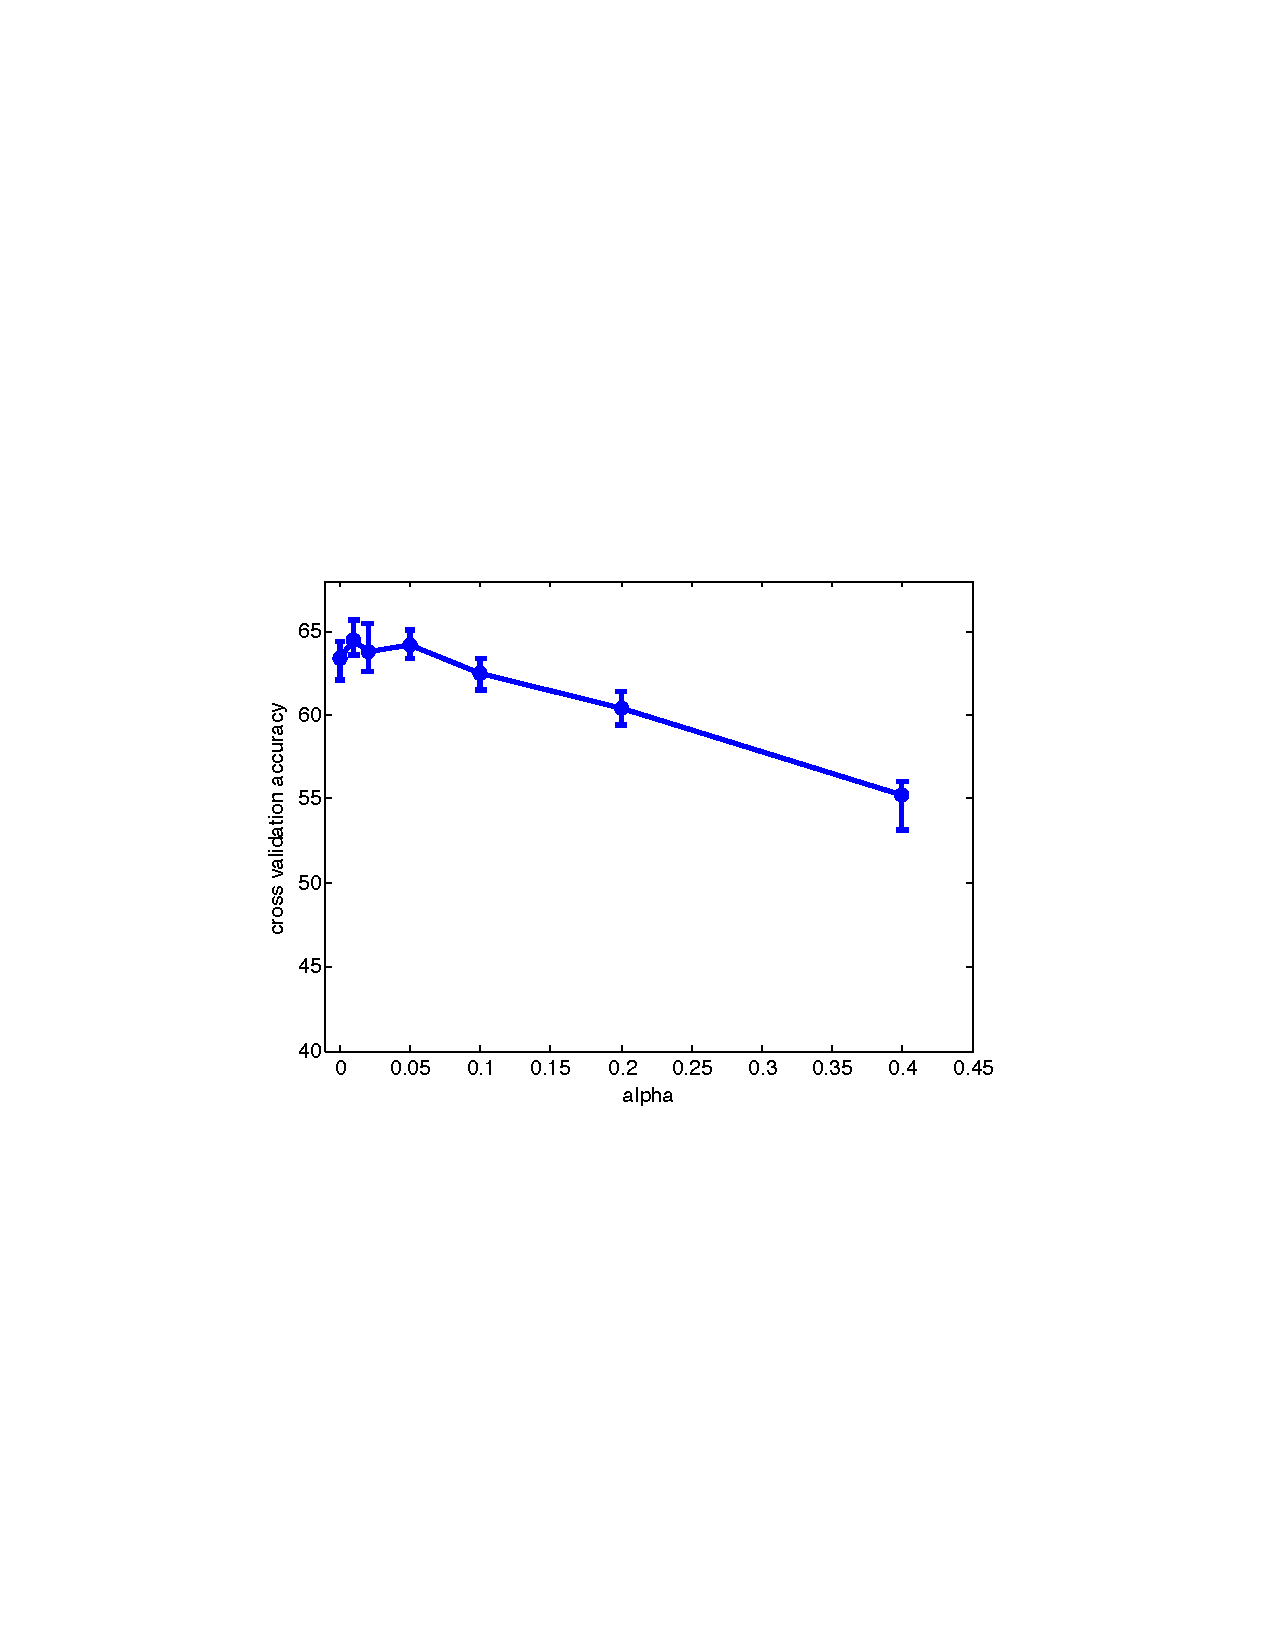
\includegraphics[width=0.45\linewidth]{alpha_plot.pdf}
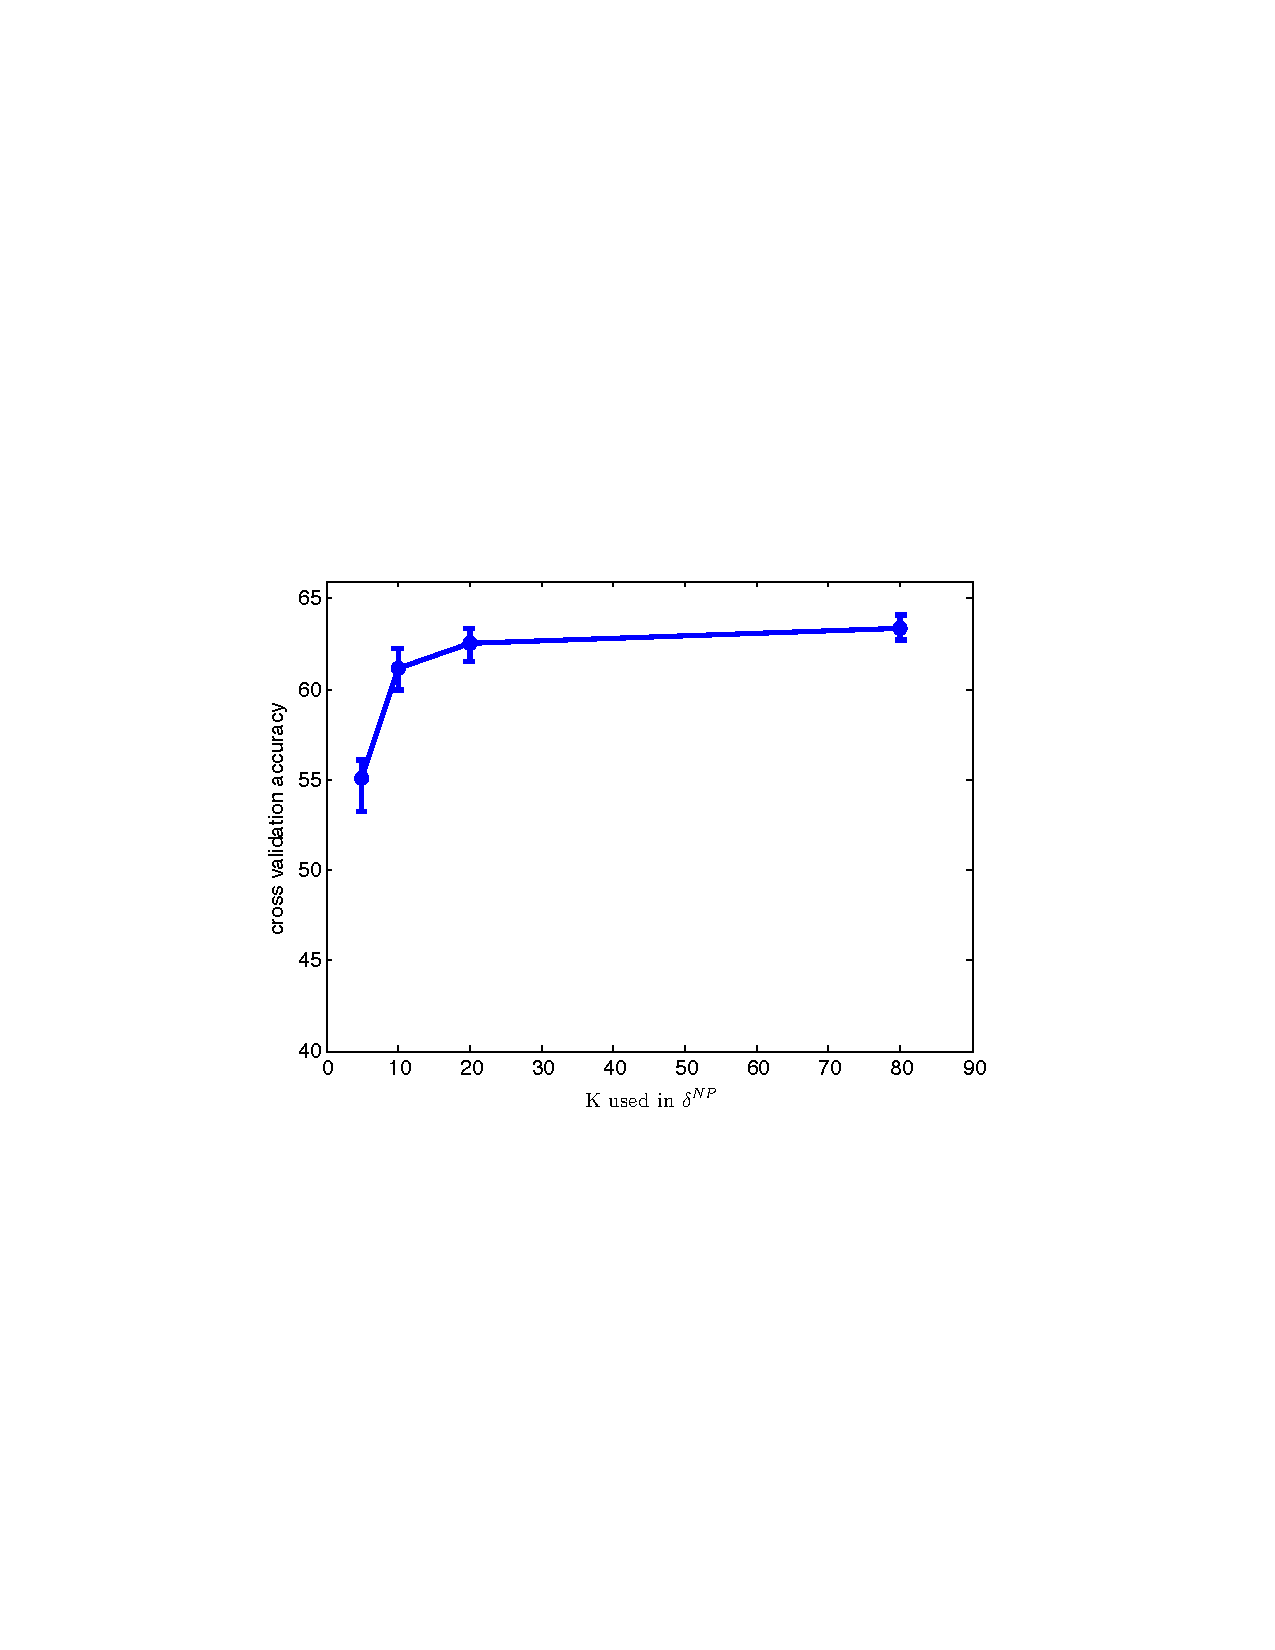
\includegraphics[width=0.45\linewidth]{K_plot.pdf}
\end{center}
\caption{Cross-validation results on fine-grained accuracy for different values of $\alpha$ (left) and $K$ (right). We split the training data into 5 folds and use cross-validate each hyperparameter setting.}
\label{fig:crossvalidationalphak}
\end{figure*}




As shown in Table \ref{tab:partlocalres}, for both settings of given bounding box and unknown bounding box, our methods outperform the strong DPM~\cite{Hossein_ECCV12} method.
Adding a geometric constraint $\delta^{NP}$ improves our results (79.82\% for body localization compared to 65.42\%). In the fully automatic setting, the top ranked detection and part localization performance on head is 65\% better than the baseline method. $\Delta_{\mathrm{null}}=1$ is the appearance-only case with no geometric constraints applied. Although the fine-grained classification results don't show a big gap between $\Delta_{\mathrm{geometric}}$ and $\Delta_{\mathrm{box}}$, we can see the performance gap for part localization.
The reason for the small performance gap might be that deep convolutional features are invariant to small translations and rotations,
limiting the impact of small localization errors on our end-to-end accuracy.


We also evaluate the recall performance of selective search region proposals \cite{selsearch} for bounding box and semantic parts. 
The results of recall given different overlapping thresholds are shown in Table \ref{tab:selective_search_recall}. 
Recall for the bird head and body parts is high when the overlap requirement is $0.5$, which provides the foundation for localizing these parts given the region proposals. However, we also observe that the recall for head is below $40\%$ when the overlap threshold is $0.7$, indicating the bottom-up region proposals could be a bottleneck for precise part localization.

Other visualizations are shown in Figure~\ref{fig:comparasion}. We show three detection and part localization for each image, the first column is the output from strong DPM, the second column is our methods with individual part predictions and the last column is our method with local prior. We used the model pretrained from \cite{Hossein_ECCV12} to get the results. We also show some failure cases of our method in Figure~\ref{fig:failure}.


\subsection{Component Analysis}
To examine the effect of different values of $\alpha$ and $K$ used in $\Delta_{\mathrm{geometric}}$, we conduct cross-validation experiments.
Results are shown in Figure~\ref{fig:crossvalidationalphak}. We fix $K=20$ in Figure~\ref{fig:crossvalidationalphak}, left and fix $\alpha = 0.1$ in Figure \ref{fig:crossvalidationalphak}, right. All the experiments on conducted on training data in a cross-validation fashion and we split the training data into 5 folds.
%\todo{can we add error bars? ... if you still have the results}.
As the results show, the end-to-end fine-grained classification results are sensitive to the choice of $\alpha$ and $\alpha=0$ is the case of $\Delta_{\mathrm{box}}$ predictions without any geometric constraints. The reason why we have to pick a small $\alpha$ is the pdf of the Gaussian is large compared to the logistic score function output from our part detectors. On the other hand, the choice of $K$ cannot be too small and it is not very sensitive when $K$ is larger than 10. 


%Experiment results vary K, vary $\alpha$
%Answer the following questions,
%1) Are parts necessary, show results with only root filter
%2) Are neighbors necssarcy, show only fit into one Gaussian
%3) Show hor prior helps, show results without prior
%
%figure to visualize the prior over neighbors v.s. prior over the whole training data


\begin{figure*}
\begin{center}
\begin{tabular}{ccc}
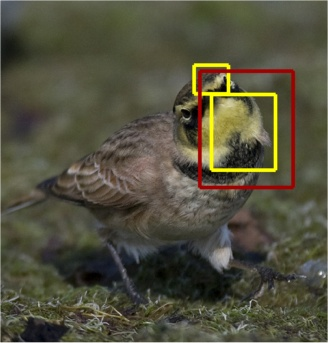
\includegraphics[width=0.3\linewidth]{6_strong_dpm.jpg} &
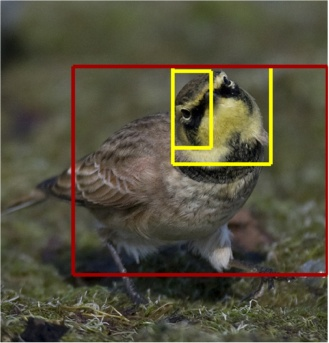
\includegraphics[width=0.3\linewidth]{6_individual.jpg} &
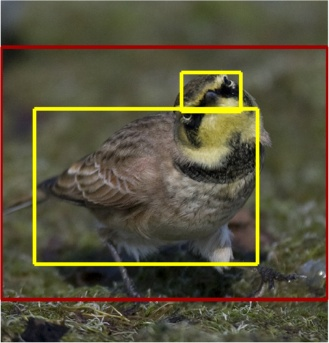
\includegraphics[width=0.3\linewidth]{6_neighbor.jpg} \\
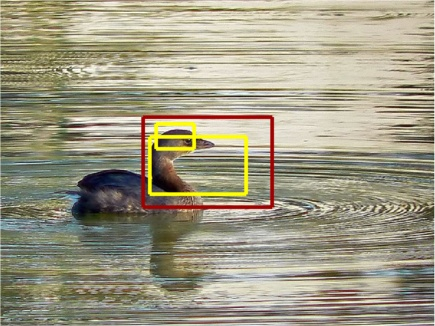
\includegraphics[trim=0mm 10mm 0mm 10mm, clip, width=0.3\linewidth]{11_strong_dpm.jpg} &
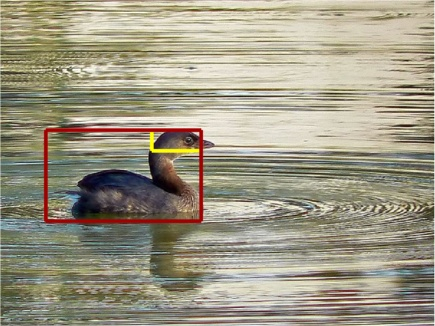
\includegraphics[trim=0mm 10mm 0mm 10mm, clip, width=0.3\linewidth]{11_individual.jpg} &
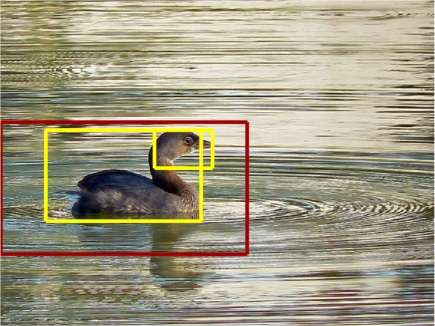
\includegraphics[trim=0mm 10mm 0mm 10mm, clip, width=0.3\linewidth]{11_neighbor.jpg} \\
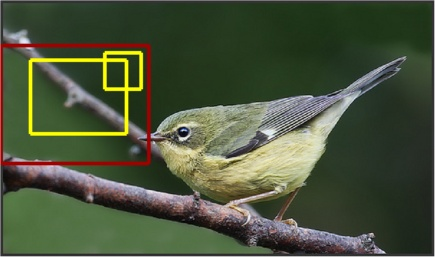
\includegraphics[width=0.3\linewidth]{13_strong_dpm.jpg} &
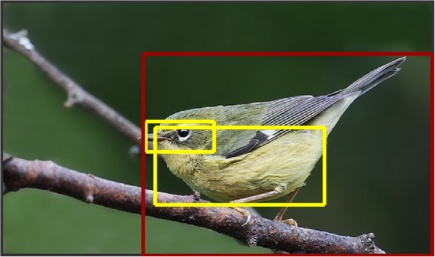
\includegraphics[width=0.3\linewidth]{13_individual.jpg} &
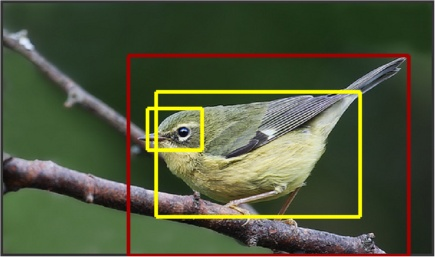
\includegraphics[width=0.3\linewidth]{13_neighbor.jpg} \\
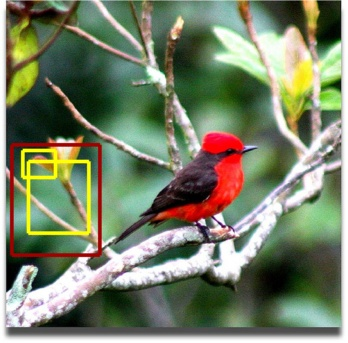
\includegraphics[trim=0mm 20mm 0mm 20mm, clip, width=0.3\linewidth]{15_strong_dpm.jpg} &
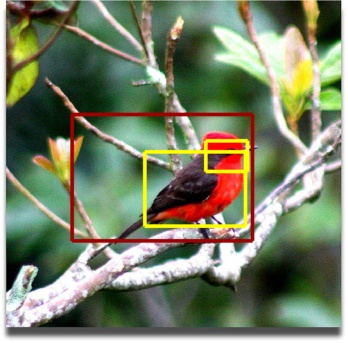
\includegraphics[trim=0mm 20mm 0mm 20mm, clip, width=0.3\linewidth]{15_individual.jpg} &
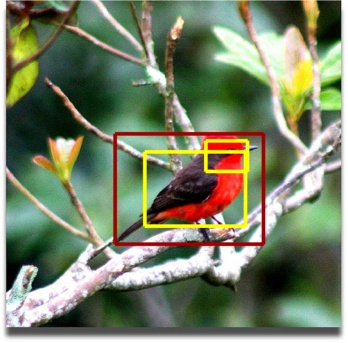
\includegraphics[trim=0mm 20mm 0mm 20mm, clip, width=0.3\linewidth]{15_neighbor.jpg} \\
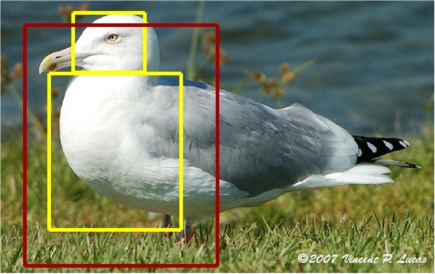
\includegraphics[width=0.3\linewidth]{16_strong_dpm.jpg} &
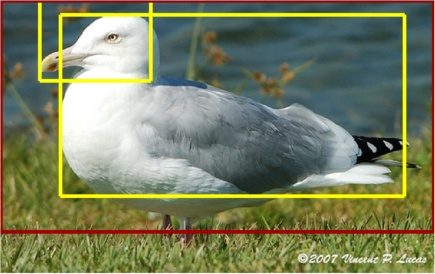
\includegraphics[width=0.3\linewidth]{16_individual.jpg} &
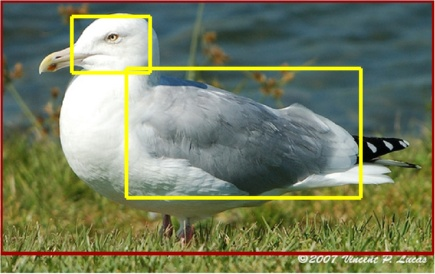
\includegraphics[width=0.3\linewidth]{16_neighbor.jpg} \\
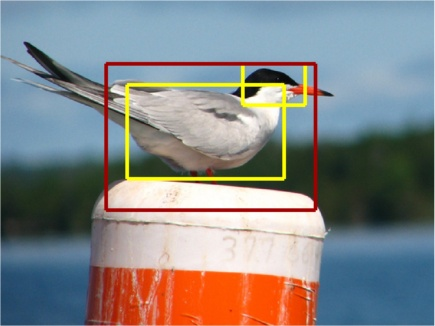
\includegraphics[width=0.3\linewidth]{17_strong_dpm.jpg} &
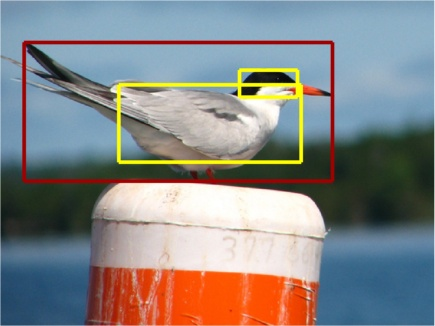
\includegraphics[width=0.3\linewidth]{17_individual.jpg} &
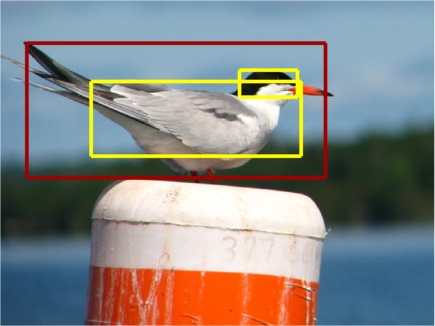
\includegraphics[width=0.3\linewidth]{17_neighbor.jpg} \\
% 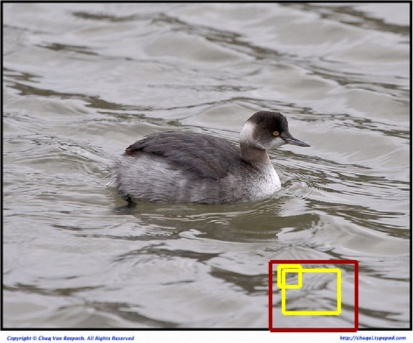
\includegraphics[width=0.3\linewidth]{19_strong_dpm.jpg} &
% 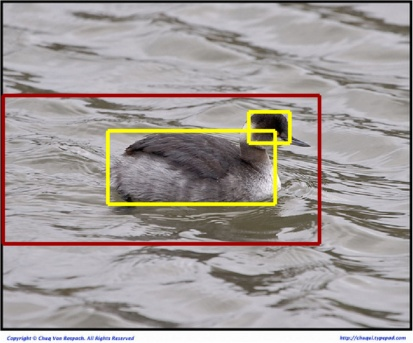
\includegraphics[width=0.3\linewidth]{19_individual.jpg} &
% 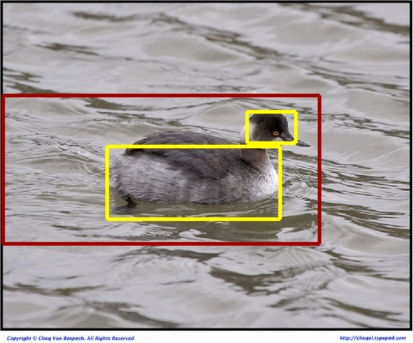
\includegraphics[width=0.3\linewidth]{19_neighbor.jpg} \\
% 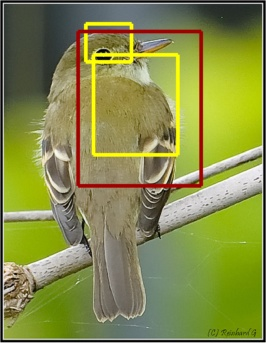
\includegraphics[width=0.3\linewidth]{30_strong_dpm.jpg} &
% 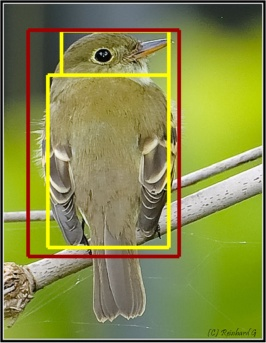
\includegraphics[width=0.3\linewidth]{30_individual.jpg} &
% 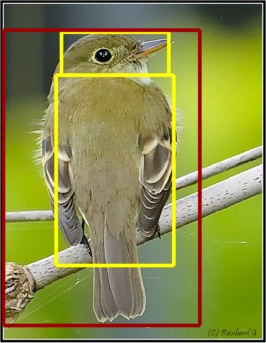
\includegraphics[width=0.3\linewidth]{30_neighbor.jpg} \\
Strong DPM & Ours ($\Delta_{box}$) & Ours ($\delta^{NP}$)
\\
\end{tabular}
\end{center}
\caption{{Examples of bird detection and part localization from strong DPM~\cite{Hossein_ECCV12} (left); our method using $\Delta_{\mathrm{box}}$ part predictions (middle); and our method using $\delta^{NP}$(right). All detection and localization results without any assumption of bounding box. }}
\label{fig:comparasion}
\end{figure*}

\begin{figure*}
\begin{center}
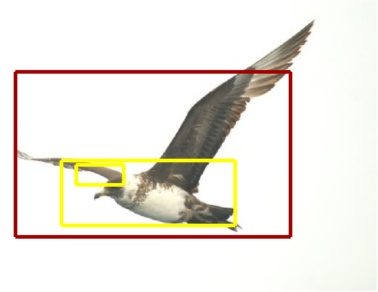
\includegraphics[height=0.2\linewidth]{8_neighbor.jpg} 
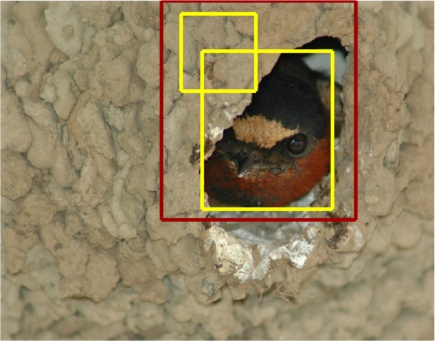
\includegraphics[height=0.2\linewidth]{32_neighbor.jpg} 
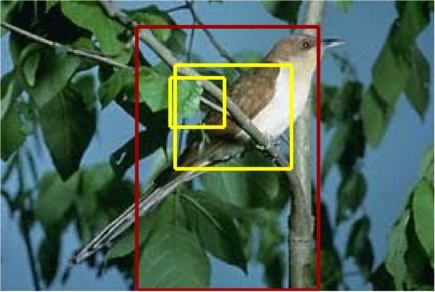
\includegraphics[height=0.2\linewidth]{41_neighbor.jpg} 
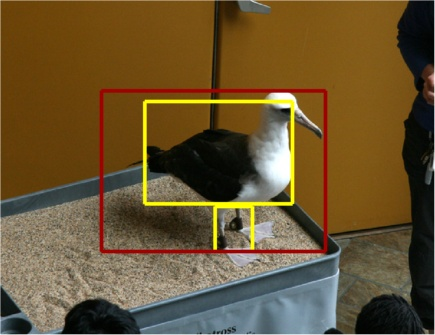
\includegraphics[height=0.2\linewidth]{57_neighbor.jpg} 
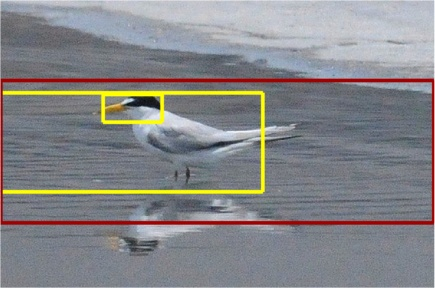
\includegraphics[height=0.2\linewidth]{58_neighbor.jpg}
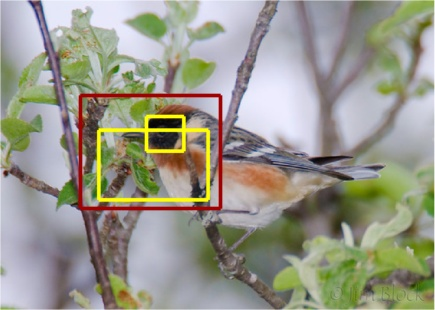
\includegraphics[height=0.2\linewidth]{64_neighbor.jpg} 
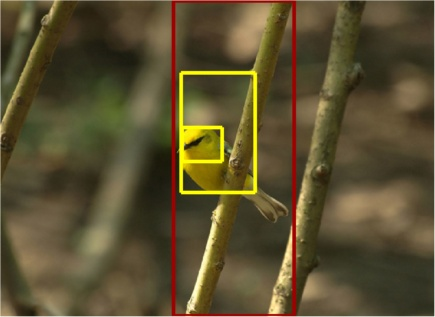
\includegraphics[height=0.2\linewidth]{99_neighbor.jpg} 
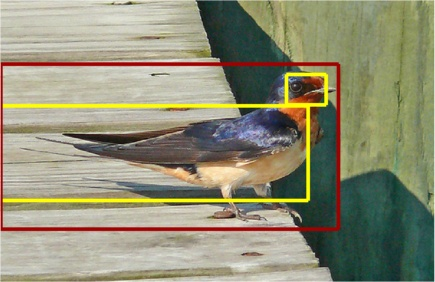
\includegraphics[height=0.2\linewidth]{47_neighbor.jpg} 
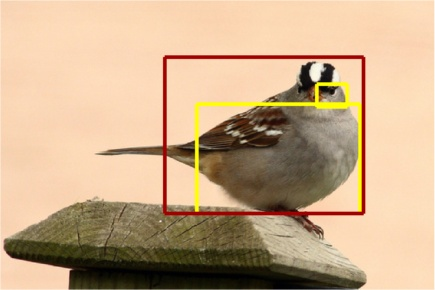
\includegraphics[height=0.2\linewidth]{91_neighbor.jpg} 
\end{center}
\caption{{Failure cases of our part localization using $\delta^{NP}$.}}
\label{fig:failure}
\end{figure*}


\section{Discussion}
\section{Discussion}
\label{sec:discussion}

The accuracy on the CKP set shows that the chosen approach is robust, misclassification usually occurs on pictures which are the first few instances of an emotion sequence. Often a neutral facial expression is depicted in those frames. Thus those misclassifications are not necessarily an error in the approach, but in the data selection. Other than that no major problem could be detected. The emotion \textit{Surprise} is often confused with \textit{Disgust} with a rate of 0.045\% which is the highest. Of those images, where an emotion is present, only few are wrongly classified.\\ 


As there is no consent for the misclassified images, they cannot be depicted here. However some unique names are provided. \\
Image S119\_001\_00000010 is classified as \textit{Fear} while the annotated emotion corresponds to \textit{Surprise}. The image depicts a person with a wide open mouth and open eyes. Pictures representing \textit{Surprise} are often very similar, since the persons also have wide open mouths and eyes. In image S032\_004\_00000014 the targeted label \textit{Fear} is confused with \textit{Anger}. While the mouth region in pictures with \textit{Anger} differ, the eye regions are alike, since in both situations the eyes and eyebrows are contracted.\\
Similar effects are experienced when dealing with the MMI Dataset. Since the first two frames are discarded most pictures with neutral positions are excluded. In few images a neutral position can still be found which gives rise to errors. For the same reason as the CKP set images will not be displayed. Due to the approach to extract images of the videos, a unique identifier for the misclassified image cannot be provided.\\
The top confusions are observed for \textit{Fear} and \textit{Surprise} with a rate of 0.0159\% where \textit{Fear} is wrongly misclassified as \textit{Surprise}. Session 1937 shows a woman displaying \textit{Fear} but it is classified as \textit{Surprise}. Both share common features like similar eye and mouth movement. In both emotions, participants move the head slightly backwards. This can be identified by wrinkled skin. The second most confusion rate, \textit{Surprise} being mistaken as \textit{Sadness}, is mostly based on neutral position images. Although the first two images are not used, some selected frames still do not contain an emotion. In Session 1985 \textit{Surprise} is being mistaken as \textit{Sadness}. The image depicts a man with his mouth being slightly curved, making him look sad.\\

DeXpression extracts features and uses them to classify images, but in very few cases the emotions are confused. This happens, as discussed, usually in pictures depicting no emotion. DeXpression performs very well on both tested sets, if an emotion is present.



\begin{figure*}
	\centering
	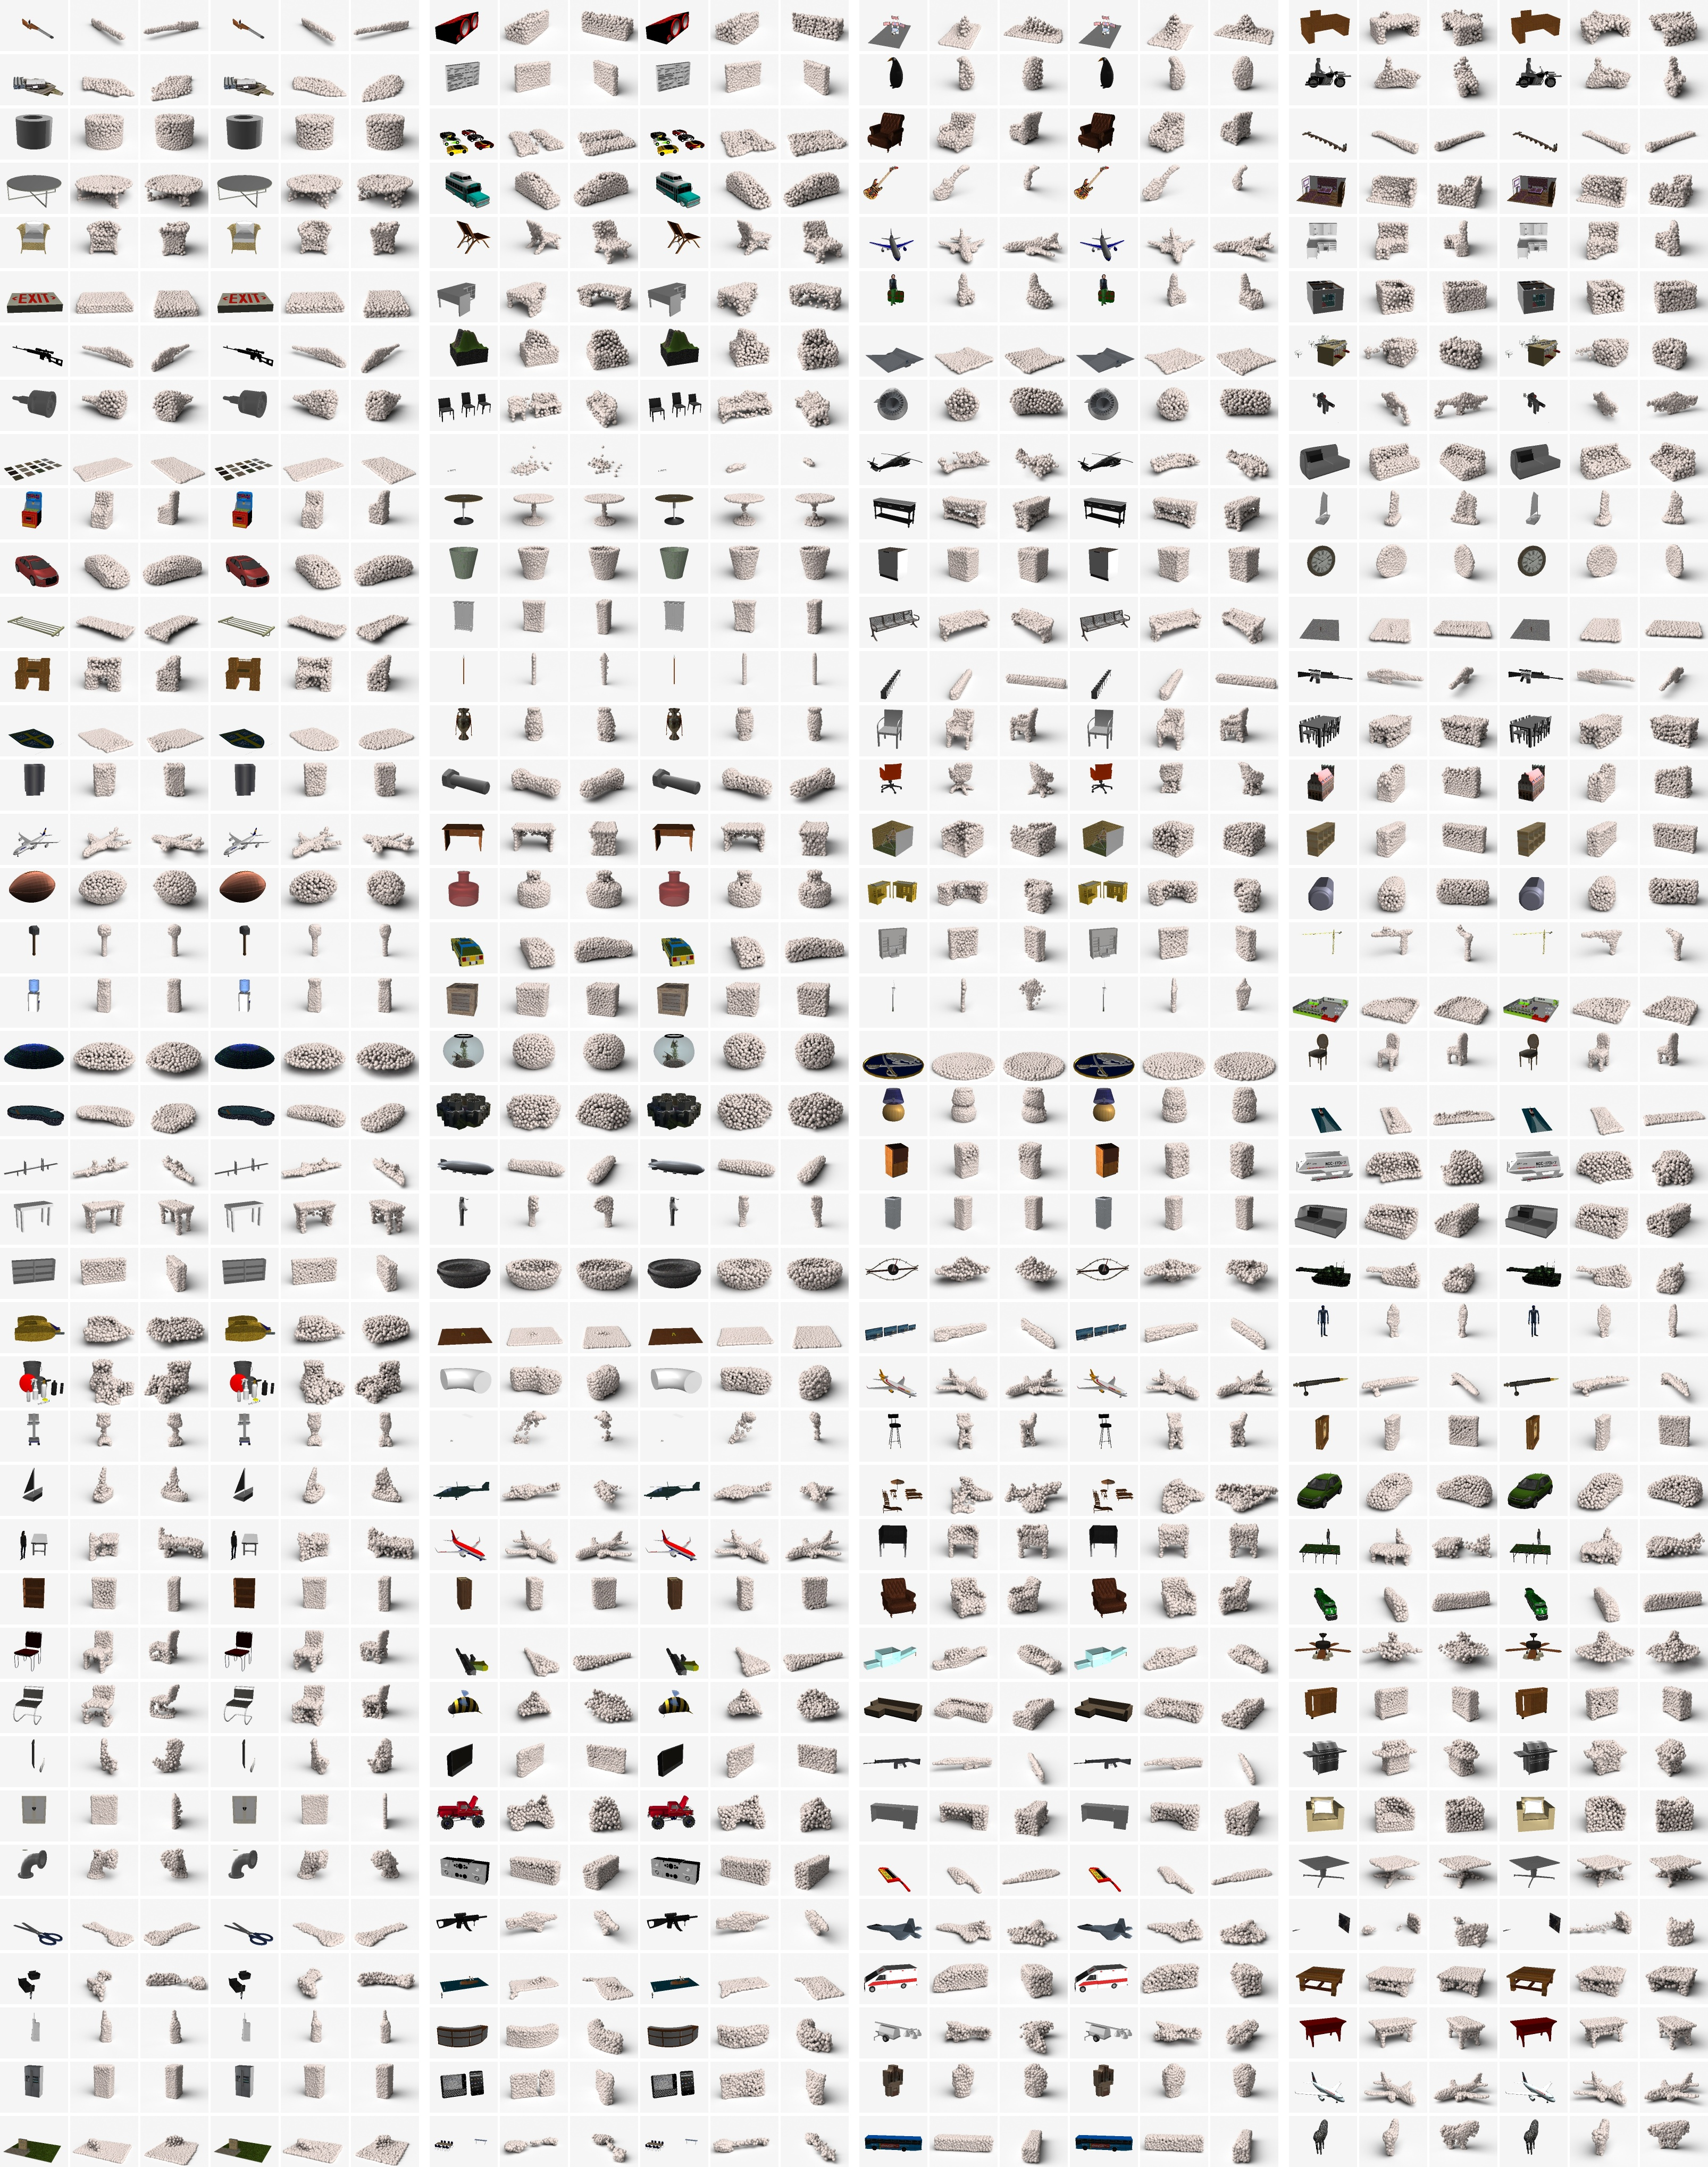
\includegraphics[width=\linewidth]{./fig/show_all_emd.jpg}
	\caption{First 5 mini-batches of our validation set. Result obtained by CD is on the left, EMD on the right.}
	\label{fig:show_all}
\end{figure*}

%\section{Conclusion}
%\label{sec:conclusion}
We introduce a novel neural network architecture, the Synchronized Spectral CNN (SyncSpecCNN), for semantic annotation on 3D shape graphs. To share coefficients and conduct multi-scale analysis in different parts of a single shape graph, we introduce a spectral parametrization of dilated convolutional kernels. To allow parameter sharing across related but different shapes that may be represented by very different graphs, we introduce a spectral transformer network to synchronize different spectral domains. The effectiveness of different components in our network is validated through extensive experiments. Jointly these contributions lead to state-of-the-art performance on various semantic annotation tasks including 3D shape part segmentation and 3D keypoint prediction.

{\bibliographystyle{ieee}
\bibliography{si2pc}
}



\end{document}
